%% GABARIT POUR THÈSE PAR ARTICLES
%%
%% Consulter la documentation de la classe ulthese pour une
%% description détaillée de la classe, de ce gabarit et des options
%% disponibles.
%%
%% [Ne pas hésiter à supprimer les commentaires après les avoir lus.]
%%
%% Déclaration de la classe avec le type de grade
%%   [l'un de LLD, DMus, DPsy, DThP, PhD]
%% et les langues les plus courantes. Le français sera la langue par
%% défaut du document. L'option 'bibsection' permet de créer des
%% bibliographies par chapitre présentées sous forme de section
%% numérotée.
\documentclass[PhD,bibsection,english,french,oldfontcommands]{ulthese}
  %% Encodage utilisé pour les caractères accentués dans les fichiers
  %% source du document. Les gabarits sont encodés en UTF-8. Inutile
  %% avec XeLaTeX, qui gère Unicode nativement.
  \ifxetex\else \usepackage[utf8]{inputenc} \fi

  %% Charger ici les autres paquetages nécessaires pour le document.
  %% Quelques exemples; décommenter au besoin.
  %\usepackage{amsmath}       % recommandé pour les mathématiques
  %\usepackage{ncccomma}      % gestion de la virgule dans les nombres

  %% Utilisation d'une autre police de caractères pour le document.
  %% - Sous LaTeX
  %\usepackage{mathpazo}      % texte et mathématiques en Palatino
  %\usepackage{mathptmx}      % texte et mathématiques en Times
  %% - Sous XeLaTeX
  %\setmainfont{TeX Gyre Pagella}      % texte en Pagella (Palatino)
  %\setmathfont{TeX Gyre Pagella Math} % mathématiques en Pagella (Palatino)
  %\setmainfont{TeX Gyre Termes}       % texte en Termes (Times)
  %\setmathfont{TeX Gyre Termes Math}  % mathématiques en Termes (Times)

\usepackage{amsmath}
\usepackage{amssymb}
\usepackage{mathtools}
\usepackage{expl3}
\usepackage{xspace}
\usepackage{graphicx}
\usepackage{makecell}
\usepackage{rotating}
\usepackage{gensymb}
\usepackage{xcolor}

\let\newfloat\undefined
\usepackage{floatrow}

\usepackage{nicefrac}
\usepackage{booktabs,tabu}

  %% Gestion des hyperliens dans le document. S'assurer que hyperref
  %% est le dernier paquetage chargé.
  \usepackage{hyperref}
  \hypersetup{colorlinks,allcolors=ULlinkcolor}

\ExplSyntaxOn
\newcommand\latinabbrev[1]{
  \peek_meaning:NTF . {% Same as \@ifnextchar
    #1\@}%
  { \peek_catcode:NTF a {% Check whether next char has same catcode as \'a, i.e., is a letter
      #1.\@ }%
    {#1.\@}}}
\ExplSyntaxOff

\DeclareMathOperator*{\argmax}{arg\,max}
\DeclareMathOperator*{\argmin}{arg\,min}

\newcommand{\boldomega}{\boldsymbol \omega} % bold omega
\newcommand{\boldmu}{\boldsymbol \mu} % bold omega
\newcommand{\bolddelta}{\boldsymbol \delta} % bold delta
\newcommand{\boldtheta}{\boldsymbol \theta}
\newcommand{\boldrho}{\boldsymbol \rho}
\newcommand{\Reals}{\mathbb{R}}

\newcommand{\etal}{\latinabbrev{et al}.}
\newcommand{\ie}{\latinabbrev{i.e.}}
\newcommand{\eg}{\latinabbrev{e.g.}}

\newcommand\norm[1]{\left\lVert#1\right\rVert}

\newcommand\todo[1]{\textcolor{red}{TODO: #1}}

\newcommand\degr[0]{^{\circ}}

\graphicspath{{figures/}, {ECCV18/}, {CVPR17/}, {CVPR18/}}

  %% Options de mise en forme du mode français de babel. Consulter la
  %% documentation du paquetage babel pour les options disponibles.
  %% Désactiver (effacer ou mettre en commentaire) si l'option
  %% 'nobabel' est spécifiée au chargement de la classe.
  \frenchbsetup{%
    StandardItemizeEnv=true,       % format standard des listes
    ThinSpaceInFrenchNumbers=true, % espace fine dans les nombres
    og=«, fg=»                     % caractères « et » sont les guillemets
  }

  %% Suppression du numéro de section de la bibliographie. Utilisation
  %% de \extrasfrench parce que c'est la dernière langue déclarée dans
  %% \documentclass, ci-dessus.
  %\addto\extrasfrench{%
  %  \renewcommand{\bibsection}{\section*{\bibname}\prebibhook}}

  %% Déclarations des pages de titre. Remplacer les éléments entre < >.
  %% Supprimer les caractères < >. Couper un long titre ou un long
  %% sous-titre manuellement avec \\.
  \titre{<Titre principal>}
  % \titre{Ceci est un exemple de long titre \\
  %   avec saut de ligne manuel}
  % \soustitre{Sous-titre le cas échéant}
  % \soustitre{Ceci est un exemple de long sous-titre \\
  %   avec saut de ligne manuel}
  \auteur{Yannick Hold-Geoffroy}
  \annee{2018}
  \direction{Jean-François Lalonde, directeur de recherche}
  \codirection{Paulo F.U. Gotardo, codirecteur de recherche}
  % \codirection{<Prénom Nom>, <codirecteur ou codirectrice> de recherche \\
  %              <Prénom Nom>, <codirecteur ou codirectrice> de recherche}

\begin{document}

\frontmatter                    % pages liminaires

\pagestitre                     % production des pages de titre

\chapter*{Résumé}                      % ne pas numéroter
\phantomsection\addcontentsline{toc}{chapter}{Résumé} % inclure dans TdM

\begin{otherlanguage*}{french}
  Texte du résumé en français.
\end{otherlanguage*}
                % résumé français
\chapter*{Abstract}                      % ne pas numéroter
\phantomsection\addcontentsline{toc}{chapter}{Abstract} % inclure dans TdM

\begin{otherlanguage*}{english}

  Understanding images is needed for a plethora of tasks, from compositing to image relighting, including 3D object reconstruction. These tasks allow artists to realize masterpieces or help operators to safely make decisions based on visual stimuli. For many of these tasks, the physical and geometric models that the scientific community has developed give rise to ill-posed problems with several solutions, only one of which is generally reasonable. To resolve these indeterminations, the reasoning about the visual and semantic context of a scene is usually relayed to an artist or an expert who uses his experience to carry out his work. This is because humans are able to reason globally on the scene in order to obtain plausible and appreciable results. Would it be possible to model this experience from visual data and partly or totally automate tasks? This is the topic of this thesis: modeling priors using deep machine learning to solve typically ill-posed problems. More specifically, we will cover three research axes: 1) surface reconstruction using photometric cues, 2) outdoor illumination estimation from a single image and 3) camera calibration estimation from a single image with generic content. These three topics will be addressed from a data-driven perspective. Each of these axes includes in-depth performance analyses and, despite the reputation of opacity of deep machine learning algorithms, we offer studies on the visual cues captured by our methods. 

\end{otherlanguage*}
              % résumé anglais
\cleardoublepage

\tableofcontents                % production de la TdM
\cleardoublepage

\listoftables                   % production de la liste des tableaux
\cleardoublepage

\listoffigures                  % production de la liste des figures
\cleardoublepage

\dedicace{Dédicace si désiré}
\cleardoublepage

\epigraphe{Texte de l'épigraphe}{Source ou auteur}
\cleardoublepage

\chapter*{Remerciements}         % ne pas numéroter
\phantomsection\addcontentsline{toc}{chapter}{Remerciements} % inclure dans TdM

- HDRDB team
- Disney team
- Adobe team
         % remerciements
%!TEX root = main.tex
\chapter*{Preface}         % ne pas numéroter
\phantomsection\addcontentsline{toc}{chapter}{Preface} % inclure dans TdM

Most of the work presented in this dissertation was published in peer-reviewed conferences between 2015 and 2018 with myself as first author. %For every publication, I developed and executed all experiments, prepared the datasets and trained all machine learning models. 


Chapter~\ref{ch1} is mostly taken from our ICCP'15~\cite{holdgeoffroy-iccp-15} and 3DV'15~\cite{holdgeoffroy-3dv-15} publications. For the latter, we received the ``Best Paper (Runner Up)'' award in Lyon. More information on both works can be found on their project pages\footnote{\url{http://jflalonde.ca/projects/outdoorPS/} and \url{http://jflalonde.ca/projects/xHourPS/}}. The work presented on chapter~\ref{ch2} has been submitted for peer review at ECCV'18; we are still awaiting updates for this submission. Chapters~\ref{ch3} and~\ref{ch4} were both published to the prestigious CVPR (158 h-index), the former as a long oral presentation~\cite{holdgeoffroy-cvpr-17} (3\% acceptance rate), and the latter as a poster~\cite{holdgeoffroy-cvpr-18} (30\% acceptance rate). More information on both can be found on their project page\footnote{\url{http://jflalonde.ca/projects/deepOutdoorLight/} and \todo{add project page}}.


%\bibliographystyle{abbrvnat}
%\bibliography{library}
           % avant-propos

\mainmatter                     % corps du document

%%!TEX root = main.tex
\section{Introduction}

\begin{figure}
\centering
\includegraphics[width=\linewidth]{figures/teaser/teaser-skymodel.pdf}
\caption[Presentation of the proposed method]{We present an approach for predicting full HDR lighting conditions from a single LDR outdoor image. Our prediction can readily be used to insert a virtual object into the image. Our key idea is to train a CNN using input-output pairs of LDR images and HDR illumination parameters that are automatically extracted from a large database of $360^\circ$ panoramas.}
\label{fig:teaser}
\vspace{-1em}
\end{figure}

Illumination plays a critical role in deciding the appearance of a scene, and recovering scene illumination is important for a number of tasks ranging from scene understanding to reconstruction and editing. However, the process of image formation conflates illumination with scene geometry and material properties in complex ways and inverting this process is an extremely ill-posed problem. This is especially true in outdoor scenes, where we have little to no control over the capture process.

Previous approaches to this problem have relied on extracting cues such as shadows and shading~\cite{lalonde-ijcv-12} and combining them with (reasonably good) estimates of scene geometry to recover illumination. However, both these tasks are challenging and existing attempts often result in poor performance on real-world images. Alternatively, techniques for intrinsic images can estimate low-frequency illumination but rely on hand-tuned priors on geometry and material properties~\cite{barron-pami-15,lombardi2016reflectance} that may not generalize to large-scale scenes. In this work, we seek a single image outdoor illumination inference technique that generalizes to a wide range of scenes and does not make strong assumptions about scene properties.

To this end, our goal is to train a CNN to directly regress a single input low dynamic range image to its corresponding high dynamic range (HDR) outdoor lighting conditions. Given the success of deep networks at related tasks like intrinsic images~\cite{zhou2015intrinsic} and reflectance map estimation~\cite{rematas-cvpr-16}, our hope is that an appropriately designed CNN can learn this relationship. However, training such a CNN requires a very large dataset of outdoor images with their corresponding HDR lighting conditions. Unfortunately, such a dataset currently does not exist, and, because capturing light probes requires significant time and effort, acquiring it is prohibitive.

Our insight is to exploit a large dataset of outdoor panoramas~\cite{xiao-cvpr-12}, and extract photos with limited field of view from them. We can thus use pairs of photos and panoramas to train the neural network. However, this approach is bound to fail since: 1) the panoramas have low dynamic range and therefore do not provide an accurate estimate of outdoor lighting; and 2) even if notable attempts have been made~\cite{zhang-cvpr-13}, recovering full spherical panoramas from a single photo is both improbable and unnecessary for a number of tasks (e.g., many of the high-frequency details in the panoramas are not required when rendering Lambertian objects into the scene).

Instead, we use a physically-based sky model---the Ho\v{s}ek-Wilkie model~\cite{hosek-siggraph-12,hosek-cga-13}---and fit its parameters to the visible sky regions in the input panorama. This has two advantages: first, it allows us to recover physically accurate, high dynamic range information from the panoramas (even in saturated regions). Second, it compresses the panorama to a compact set of physically meaningful and representative parameters that can be efficiently learned by a CNN. At test time, we recover these parameters---including sun position, atmospheric turbidity, and geometric and radiometric camera calibration---from an input image and use them to construct an HDR sky environment map. 

To our knowledge, we are the first to address the complete scope of estimating a full HDR lighting representation---which can readily be used for image-based lighting~\cite{Debevec1998}---from a single outdoor image (fig.~\ref{fig:teaser}). Previous techniques have typically addressed only aspects of this problem, e.g., Lalonde et al.~\cite{lalonde-ijcv-12} recover the position of the sun but need to observe sky pixels in order to recover the atmospheric conditions. Similarly,~\cite{Ma2017} uses a neural network to estimate the sun azimuth to perform localization in roadside environments. Karsch et al.~\cite{karsch2014automatic} estimate full environment map lighting, but their panorama transfer technique may yield illumination conditions arbitrarily far away from the real ones. In contrast, our technique can recover an accurate, full HDR sky environment map from an arbitrary input image. We show through extensive evaluation that our estimates of the lighting conditions are significantly better than previous techniques and that they can be used ``as is'' to photorealistically relight and render 3D models into images.    




\chapter{Titre du chapitre}     % numéroté

Texte du chapitre.

\bibliographystyle{}              % style de la bibliographie
\bibliography{}                   % production de la bibliographie

\chapter{Titre du chapitre}     % numéroté


%!TEX root = main.tex
\section{Introduction}

Despite nearly 40 years of study, the biggest challenge in outdoor Photometric Stereo (PS) remains the fact that the sun, our main light source, moves along a trajectory that nearly lies on a plane throughout the course of the day, leaving the photometric reconstruction under-constrained~\cite{woodham-opteng-80}.
%Researchers have investigated different approaches to address this problem, which include collecting data for several months~\cite{abrams-eccv-12,ackermann-cvpr-12}, waiting for the best time of the year (around summer solstice in the North Hemisphere~\cite{shen-pg-14}) or, more recently, for a day with favorable atmospheric conditions (partly cloudy sky~\cite{holdgeoffroy-iccp-15,holdgeoffroy-3dv-15}).
As previously discussed, one way to circumvent this issue is to wait for partially cloudy days for the effective lighting direction to shift away from the solar plane.
In general, the practitioner has no control over the sun or the atmosphere and is therefore left with two options: ($i$) a potentially long wait for the ideal conditions to arise; or ($ii$) the use of a smarter reconstruction technique that does not rely solely on the photometric cue.

In this chapter, we investigate the second option above. By using machine learning to aggregate prior knowledge on the geometry and reflectance of common classes of objects, we aim to resolve the ambiguities cause by the limited photometric cues available in single-day outdoor PS. To avoid restricting the algorithm to a small family of objects, we build knowledge on local geometry based on the fact that complex surfaces are made up of simpler, piecewise smooth patches. Our approach is further motivated by the fact that material properties are also locally correlated within small surface patches. Working with a broad class of small surface patches keeps the approach general and also facilitates the collection of data for machine learning.

% While non-convolutional deep learning was already used in fully-constrained, indoor PS (mostly to learn a generic, ``inverse BRDF'' function)... 

As we reason in terms of surface patches, a natural choice is to follow a deep learning approach with a novel convolutional neural network (CNN) architecture to automatically learn features from image patches and guide 3D normal estimation. To our knowledge, this is the first CNN to address the problem of under-constrained, single-day outdoor PS.

Our CNN design seeks a balance between fully-calibrated PS (too restrictive) and uncalibrated PS (which introduces further ambiguities). We follow a semi-calibrated outdoor PS approach and only assume that: (1) the object is imaged at roughly predefined times of the day; (2) the sun is unobstructed by clouds at these times; and (3) an orthographic camera facing approximately north (or south). The latter assumption could be relaxed using recent advances on sun position estimation in the wild to automatically detect the camera orientation. One could then train our model on multiple camera calibrations and select the right one according to the detected orientation. Of note, our approach does not require known sun intensities nor complete geolocation data, as in previous work on outdoor PS~\cite{jung-cvpr-15}. Together, our assumptions define an ``8-figure'' subspace for the position of the sun through the year, known as an {\em analemma}, whose shape also varies with geographical location (fig.~\ref{fig:solar-analemma}).

% (PG: that's an assummed/given condition)
% camera (pointing north, orthographic projection)

% analemma (Wikipedia): position of the Sun in the sky over the course of a year, as viewed at a fixed time of day and from a fixed location on the Earth

Therefore, our outdoor PS network is required to learn priors not only on object materials and local geometry (diffuse, specular, smooth, ...), but also priors on lighting (variability in sun intensity and elevation with respect to geolocation and time of year). This knowledge is encoded in the network, which learns to output 3D normals as a non-linear function of input image patches taken throughout a day. This rich prior knowledge allows us to obtain a reconstruction performance that outperforms the current state-of-the-art on real lighting data with only 3 images, which is much lower than the 6-18 typically used by previous work~\cite{yu-iccp-13,jung-cvpr-15}. Our fully trained method will be made publicly available.

%To train our CNN, we realistically render synthetic datasets with a large variety of image patches with different geometry, materials and lighting.

%\todo{Say something about the quality of our results vs state of the art.}

We summarize our contributions as follows:
\begin{itemize}
	\item a state-of-the-art method for single-day photometric stereo on sunny days that is robust to shadows, specularities and arbitrary but uniform albedo;
    \item a pipeline to generate synthetic images with a mix of Lambertian and glossy materials that captures the diversity of real outdoor lighting.
\end{itemize}


%!TEX root = main.tex
\section{Related work}

This section focuses on the more relevant work on outdoor PS, for conciseness. For an overview of general PS, the reader is referred to the recent, excellent review in~\cite{shi-tpami-18}.

% solar plane, nearly singular (ill-conditioned) light matrix, 2-image PS
% regularization breaks at (sharp) surface discontinuities

As shown in Woodham's seminal work~\cite{woodham-opteng-80}, for Lambertian surfaces, calibrated PS computes a (scaled) normal vector in closed form as a simple linear function of the input image pixels; this linear mapping is only well-defined for images obtained under three or more (known) non-coplanar lighting directions.
% webcams, solar plane
Subsequent work on outdoor PS has struggled to meet this requirement since, over the course of a day, the sun shines from directions that nearly lie on a plane. These co-planar sun directions then yield an ill-posed problem known as two-source PS; despite extensive research using integrability and smoothness constraints~\cite{onn-ijcv-90,hernandez-pami-11}, results still present strong regularization artifacts on surfaces that are not smooth everywhere. To avoid this problem in outdoor PS, authors initially proposed gathering months of data, watching the sun elevation change over the seasons~\cite{abrams-eccv-12,ackermann-cvpr-12}. More recently, Shen~{\em et al.}~\cite{shen-pg-14} noted that the coplanarity of the daily sun directions actually varies throughout the year, with single-day outdoor PS becoming more ill-posed at high latitudes near the winter solstice, and worldwide near the equinoxes.

% single day, ditch the even with a point light source model

% richer lighting models
To compensate for limited sun motion, other approaches use richer illumination models that account for additional atmospheric factors in the sky. This is done by employing (hemi-)spherical environment maps~\cite{debevec-siggraph-98} that are either real sky images~\cite{yu-iccp-13,shi-3dv-14,hung-wacv-15} or synthesized by parametric sky models~\cite{inose-tcva-13,jung-cvpr-15}. Using a large database of real sky images, Hold-Geoffroy~{\em et al.}~\cite{holdgeoffroy-iccp-15} showed that partly cloudy days are in fact better for single-day outdoor PS since clouds obscure and further scatter sun light, causing an out-of-plane shift in the effective direction of illumination. Subsequently~\cite{holdgeoffroy-3dv-15}, they also showed that good cloud coverage conditions for stable solutions may be observed in the sky within very short time intervals of just above one hour.

Despite these developments, state-of-the-art approaches in calibrated~\cite{yu-iccp-13} and semi-calibrated~\cite{jung-cvpr-15} (based on precise geolocation) outdoor PS are still prone to potentially long waits for ideal conditions to arise in the sky; and verifying the occurrence of such events is still a trial-and-error process. These facts have motivated our goal of developing a smarter approach that uses deep learning techniques to resolve ambiguities in outdoor PS by aggregating prior knowledge on object geometry, material and their interaction with natural outdoor illumination. The approach we propose is the first of its kind; so far, deep PS had only been applied in indoor scenarios with rich and controlled illumination~\cite{yu-iccv-17,santo-iccv-17,taniai-arxiv-18,shi-tpami-18}, focusing on learning inverse functions for non-Lambertian reflectances.

%\cite{yu-iccv-17,santo-iccv-17,taniai-arxiv-18} Deep learning methods applied to photometric stereo (not one-day)

% Talk about DiLiGent~\cite{shi-tpami-18}? (Their objects have homogeneous material, with piecewise constant albedo, our method would work with any albedo pattern using the division trick. Also, only normal maps, no 3D models. Their sampling of 96 lighting directions does not approximate well the path of the sun through a day.)

% single image (nishino, deep learning)
Finally, under more extreme ambiguity, techniques for shape-from-shading (SfS)~\cite{oxholm-eccv-12,johnson-cvpr-11,barron-pami-15} attempt to recover 3D normals from a single input image, in which case the shading cue alone is obviously insufficient to uniquely define a solution. Thus, SfS relies strongly on priors of different complexities and deep learning is quickly bringing advances to the field~\cite{eigen-iccv-15,shu-cvpr-17,wu-nips-17}. While this is encouraging, here we seek to improve the accuracy of 3D normal estimation by relying less heavily on priors and more strongly on the photometric cues obtained from multiple images. In addition, we also avoid restricting the approach to a specific type of object and reflectance model ({\em e.g.}, human faces, Lambertian~\cite{shu-cvpr-17}).

% deep learning PS and shape from shading, which rely on machine learning and priors, relate to original linear mapping in PS above.}
%
% This section could end by motivating the CNN: learning spatial priors is important.


% Move these to Sec 3-4 to further motivate CNN?
%
% Although there exists a closed-form least squares solution to the simplest Lambertian surfaces, such ideally diffuse materials rarely exist in the real word. Photometric stereo for surfaces with unknown general reflectance properties (i.e., bidirectional reflectance distribution functions or BRDFs) still remains as a fundamental challenge (Shi
%
% We know from data-driven, calibrated Lambertian PS that albedo and normals are obtained as a linear mapping from the input pixels. Here we relax the Lambertian and fully calibrated assumptions to learn a more generic, nonlinear mapping for recovering normal maps outdoors.
%
% Relate to 2-image PS problem early on? But that is for Lambertian case!
%
% Thus, 3D normal estimation based solely on the photometric cue remains under-constrained, even with strong assumptions of Lambertian reflectance and fully-calibrated illumination (the well-studied 2-image PS problem~\cite{}). 


%\section{Image formation model}

% Establish basic notation/formulation but only enough background as needed to support CNN-based method in next section...


% Linear and Lambertian assumptions
% We consider a small planar surface with normal vector $\mathbf{n} \in \mathbb{R}^3$ and Lambertian reflectance with albedo $\rho$. Under Lambertian assumption, all incoming lighting from the visible hemisphere can be formulated as a single point light source, the \emph{mean light vector} $\mathbf{\bar{l}­} \in \mathbb{R}^3$~\cite{holdgeoffroy-iccp-15,hung-wacv-15}.

% Given $m$ intensity observations of the same surface $b_1, b_2, ... b_m \in \mathbb{R}$ taken at different times of the day, yielding different mean light vectors $\mathbf{\bar{l}}_1, \mathbf{\bar{l}}_2, ... \mathbf{\bar{l}}_m \in \mathbb{R}^3$, we collect all photometric constraints for that pixel and obtain the PS equation in matrix form:
% \begin{equation}
%     \mathbf{b} = 
%     \begin{bmatrix}
%     b_1 \\
%     b_2 \\
%     \vdots \\
%     b_m
%     \end{bmatrix}
%     =
%     \begin{bmatrix}
%     \mathbf{\bar{l}}_1^T \\
%     \mathbf{\bar{l}}_2^T \\
%     \vdots \\
%     \mathbf{\bar{l}}_m^T
%     \end{bmatrix}
%     \mathbf{x}, = \rho\mathbf{Lx} \;,
% \label{eq:ifm}
% \end{equation}
% where $\mathbf{x} \in \mathbb{R}^3$ is the surface normal $\mathbf{n}$ scaled by the albedo $\rho$.

% The goal of PS is to recover the surface normal $\mathbf{n}$ from the pixel intensities $\mathbf{b}$ by solving eq.~\eqref{eq:ifm}. As discussed in~\cite{holdgeoffroy-3dv-15}, the uncertainty of the recovered surface normal is proportional to the conditioning of the lighting matrix $\mathbf{L}$.

% Throughout a clear day, the sun pursue a coplanar trajectory in the sky, yielding a poorly conditioned lighting matrix $\mathbf{L}$.

%\todo{Maybe we only briefly mention this in related work, unless the CNN builds on top of it (e.g., can we claim that often clouds cause small MLV shift, but still nearby the analema?). MLV implies Lambertian and we want to relax this limitation. Also, we have a directional light model now (don't we?), not a full envmap anymore.}

% 2-source PS is an approximation of single-day with Lambertian model, pt light

% \todo{Only add stuff that helps explain/motivate CNN in next section, so likely better to start writing Sec.4 first.}

% \todo{describe preliminaries for albedo division trick here?}

%!TEX root = main.tex
\section{Deep outdoor Photometric Stereo network}
\label{sec:proposed_method}

This section presents our CNN-based approach designed to address ambiguities that arise in single-day outdoor PS reconstruction. It does so by using deep learning to model prior knowledge on object geometry, material properties, as well as their local spatial correlation and interaction with natural sky light. In order to build such knowledge base, one needs a large number of images depicting various objects lit by outdoor lighting throughout the day, over different geographic locations and days over the year; finally, the surface normal map of each object is also required. Unfortunately, no such large-scale dataset currently exists, so a natural choice is to synthesize realistic data to train our network. We begin by presenting our problem formulation, CNN architecture, followed training procedure and data generation.

\subsection{Image formation model} % includes illumination subspace (analemmata)

% sky model can represent sun position, turbidity, etc... but not clouds, that's why we assume clear skies

% BRDF can be any family, we chose isotropic GGX which is popular these days...

Consider an image pixel that depicts a small area of an object's surface, with a normal vector ${\bf n} \in \Reals^3$ and material reflectance described by a bidirectional reflectance distribution function (BRDF) $\rho(\cdot)$. When viewed from direction \mbox{${\bf v} \in \Reals^3$}, the RGB color ${\bf b}_t \in \Reals^3$ of this pixel at daytime $t$ is modeled as
%
\begin{equation}
{\bf b}_t = \int_{\Omega_{\bf n}} \rho(\boldomega, {\bf v}, {\bf n}) {\bf  L}_t(\mathbf{\boldomega}) (\boldomega^T{\bf n}) V(\boldomega) d\omega \,,
\label{eq:ifm_singlepixel}
\end{equation}
%
where $\boldomega$ is a direction of incoming light within the hemispherical domain $\Omega_{\bf n}$, ${\bf L}_t(\mathbf{\boldomega})$ is the RGB intensities (color) of the incoming light at time $t$, and $V(\boldomega)$ is a binary visibility encoding self-shadowing. Here $t$ denotes the {\em actual solar time} at the target object location.

Our goal is to invert the above rendering equation and recover the surface normal ${\bf n}$ based on the observed changes in pixel intensities ${\bf b}_t$, which are caused by the changing natural illumination ${\bf L}_t(\mathbf{\boldomega})$ as $t$ varies throughout the day. However, as discussed above, a solution based solely on the photometric cue is rarely uniquely defined and stable in outdoor PS due to the limited motion of the sun, leading to insufficient variability in ${\bf L}_t(\mathbf{\boldomega})$ and, thus, ${\bf b}_t$~\cite{holdgeoffroy-3dv-15}.

Therefore, instead of considering a single pixel $\mathbf{b}_t$, we reformulate our goal and instead aggregate additional RGB image data within a \emph{neighborhood} ${\bf B}_t \in \Reals^{16 \times 16 \times 3}$, depicting a larger surface patch centered at the pixel $\mathbf{b}_t$. Now we seek to learn a predictor ${\bf N} = f({\bf B}_{t_1}, \ldots, {\bf B}_{t_T})$, where $T$ denotes the number of input images and ${\bf N} \in \Reals^{16\times 16\times 3}$ has the patch normals. For the present work, $T=8$ but we experiment with other values in sec.~\ref{sec:ablation_study}. This approach is motivated by the fact that complex object geometry is often made up of simpler, small surface patches presenting highly correlated surface normals and material properties. A natural way to obtain this predictor $f(\cdot)$ is to train a CNN that learns a nonlinear function of local surface features that are highly correlated with the normal ${\bf n}$ at the center of the patch. We train our network on a large synthetic database of surface patches realistically rendered with a standard GGX shader for $\rho(\cdot)$, with varying diffuse and specular parameters, and using the Ho\v{s}ek-Wilkie physically-based sky model~\cite{hosek-siggraph-12} for the spherical function ${\bf L}_t(\mathbf{\boldomega})$, as described next.

%\eqref{eq:ifm_singlepixel} is non-linear due to the reflectance function, and  and approximating the 2-source PS problem. Both issues can solved by learning priors that extend the photometric constraints.

% ambiguity, normals are locally correlated within a patch
% semi-calibrate, we don't require a light probe...
% assumptions... then architecture

% clouds, as long as don't obscure sun, change predominant direction of illumination considerably far from analemmata subsbace in Fig, should be ok. See experiments for sensitivity analysis.


\subsection{Illumination model: the solar analemma}
\label{sec:analemma}

We follow a semi-calibrated PS approach that does not require known lighting environments~\cite{yu-iccp-13} nor complete camera geolocation data~\cite{jung-cvpr-15}. Our method only assumes that: (1) the object images are captured at roughly predefined times of the day, $t \in \{t_1, t_2, \ldots, t_T \}$; (2) the sun is unobstructed by clouds at these times; and (3) the camera is orthographic and faces approximately North (or South). We later (sec.~\ref{sec:analysis}) analyze the robustness of our network with respect to departures from these ideal conditions and discuss how assumption~(3) can be relaxed.

Together, these assumptions constrain the sun position to lie within an ``8-figure'' subspace at each time $t$, known as a solar {\em analemma}, whose shape also varies with geographical location (fig.~\ref{fig:solar-analemma}). For a given time $t$, the sun may be positioned at different locations depending upon the selected date and latitude, as prescribed by the analemma. The neural network is thus expected to adapt to this (constrained) variability in sun position and associated intensity. As shown in fig.~\ref{fig:solar-analemma}-(a,b), for a given timestamp and latitude, the sun position spans relatively small angular ranges, which still remain quite constrained even when considering geographical locations sampled over the Northern Hemisphere (fig.~\ref{fig:solar-analemma}-(c)) (note that a similar plot would be obtained by sampling the Southern Hemisphere with the camera facing south). 

% On sunny days, illumination can change greatly depending on the geographical location of the observer and the date. On rare occasions, it can even provide sufficient contraints for photometric stereo~\cite{shen-pg-14}.

% One of the most notable effect is the solar analemma, namely the path of the sun in the sky throughout the year as viewed at a fixed time of day. Some analemmata like the ones shown in fig.~\ref{fig:sun_positions} exhibit over 45 degrees of azimuthal range through the year, especially early morning and late afternoon. This effect is different on the zenithal angle, where a variation similar in amplitude can be witnessed around noon. As the sun is the dominant light source on a sunny day, modeling this pattern can give hints to reason on the observed scene.

% This variability of the world over the course of a day is not accurately captured by currently available outdoor photometric stereo datasets. 

\begin{figure}[t]
    \centering
    \begin{tabular}{c@{\extracolsep{\fill}}cc}
        \includegraphics[width=0.34\linewidth]{figures/sun_pos/sunpos_paris.pdf} &
        \includegraphics[width=0.34\linewidth]{figures/sun_pos/sunpos_nt.pdf} &
        \makecell[t]{\includegraphics[width=0.29\linewidth]{figures/sun_pos/sunpos_all.pdf} \vspace{-5pt}\\
        \hspace{3pt}\includegraphics[width=0.22\linewidth]{figures/sun_pos/colorbar_sunpos_prob_horizontal.pdf}} \\
        \hspace{-11pt}(a) & \hspace{-11pt}(b) & \hspace{3pt}(c)
    \end{tabular} \\
    \caption[Solar analemma: position of the sun in the sky]{Solar analemma: position of the sun in the sky at a specific time of the day and throughout a year over (a) Paris and (b) the Tropic of Cancer. Note how the analemmas spread over a wide range of zenith and azimuth angles over the course of a year. (c)~Probability of the sun location in the sky for our training set.}
    \label{fig:solar-analemma}
\end{figure}

% Solar analemma: position of the Sun in the sky over the course of a year, as viewed at a fixed time of day and from a fixed location on the Earth

The physically-based parametric sky model of Ho\v{s}ek and Wilkie~\cite{hosek-siggraph-12} is used to obtain the spherical illumination function ${\bf L}_t(\mathbf{\boldomega})$ in eq.~\eqref{eq:ifm_singlepixel}. The model represents the spectral sky radiance as a parametric function of the sun position, sky turbidity and ground albedo. Here, turbidity is set to 2, which corresponds to a clear day, and ground albedo to 0.3. Note that we do not model light scattering caused by clouds obscuring the sun and thus assume the sun is fully visible in the sky.

\subsection{Network architecture}
\label{sec:architecture}

We now turn to the design of the function ${\bf N} = f({\bf B}_{t_1}, \ldots, {\bf B}_{t_T})$ introduced above, which is done through a Convolutional Neural Network (CNN). An overview of its proposed architecture is shown in fig.~\ref{fig:architecture}. The network takes $T=8$ input $16 \times 16$ image patches, extracted from 8 images captured at regular intervals $\Delta t$ between 9:00 and 16:00 solar time throughout a single sunny day. The first layer is composed of 32 channels of $5 \times 5$ filters with shared weights across the 8 inputs. The resulting feature maps are subsequently concatenated in a single $14 \times 14 \times 256$ feature tensor. A second convolutional layer is then used, yielding 256 channels, followed by 3 residual blocks as defined in the resnet-18 architecture~\cite{he-cvpr-16}. Lastly, 2 fully-connected layers (FC) are used to produce a $16 \times 16 \times 3$ patch of estimated normals $\mathbf{n}$. Note that we experimented with fully-convolutional architectures~\cite{taniai-arxiv-18} but found the FC layers to yield better results. The ELU activation function~\cite{clevert-iclr-16} is used at every convolutional and fully connected layer, except the output layer where a $\tanh(\cdot)$ function is used. Batch normalization~\cite{ioffe-icml-15} is applied at every layer except the first one and the output layer, where it could otherwise break low-level feature detectors and output distributions.

% The architecture mix of standard feed-forward convolutional and residual layers to learn the relationship between surface normals and photometric cues exhibited throughout a single day. 
% One particularity of our architecture is the large quantity of input heads of our CNN. 

\begin{figure}[t]
	\centering
	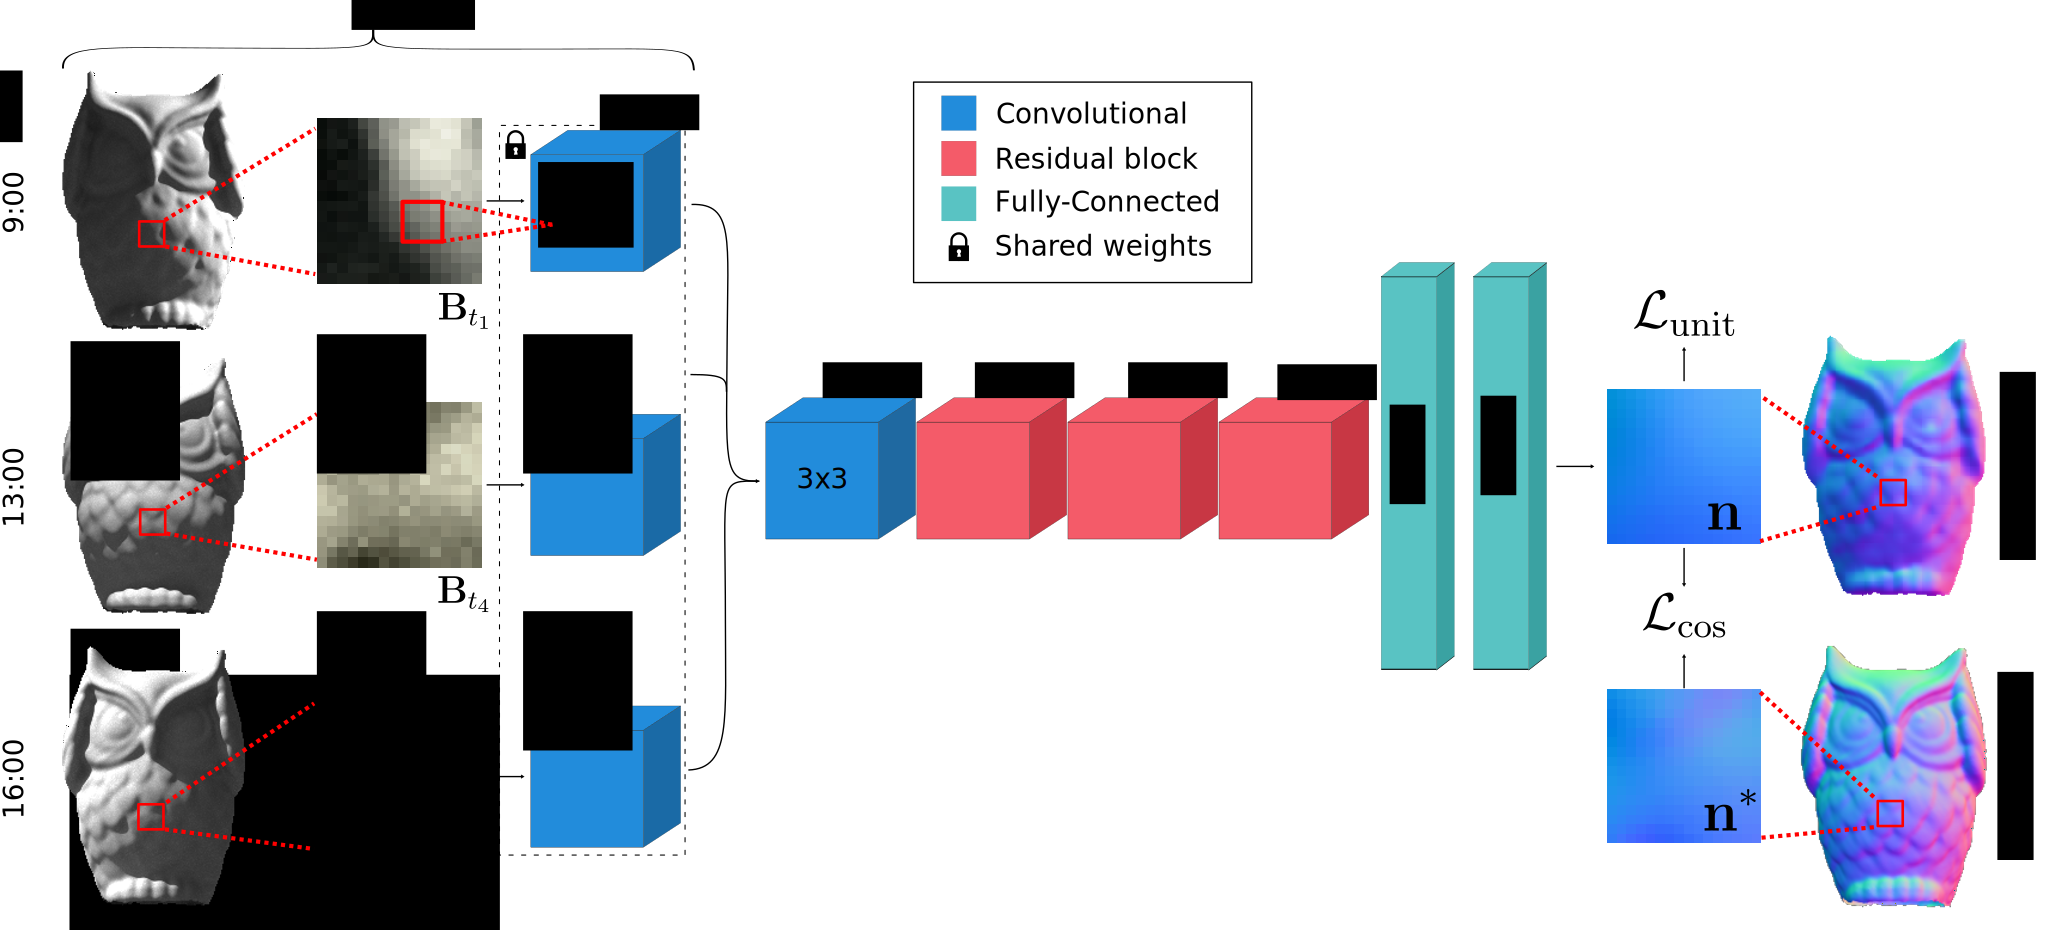
\includegraphics[width=0.8\linewidth]{figures/architecture.pdf}
	\caption[Method overview and model architecture]{Our novel CNN architecture for deep single-day outdoor PS on sunny days. The network operates on $16 \times 16$ patches $\mathbf{B}_t$ of the input image, captured at 8 time intervals $t$ regularly spaced throughout a single day. The network uses convolutional (blue) and residual (red) layers before estimating the normals using fully-connected layers (green). Two losses are used to train our method, one based on the cosine distance with the ground truth $\mathbf{\hat{n}}$ and another to constrain the norm of the output vector.}
	\label{fig:architecture}
\end{figure}

%, when photometric cues alone do not yield enough information for stable reconstruction. Using 8 input images captured at predefined times $t$ at regular intervals throughout a single sunny day, our convolutional architecture provides state-of-the-art results. We make two key observations: 1) spatial priors should be learned to overcome the weak conditioning induced by the single-day constraint, 2) to help generalization to new objects and limit the size of the training set, those spatial priors should be \emph{local}. 

The $16 \times 16$ estimated normals are represented by cartesian $(x,y,z)$ components of the surface normal of the input patch. We experimented with both cartesian $(x,y,z)$ and spherical coordinates $(\theta,\phi)$ parameterization, but found the cartesian parameterization to be more stable despite its additional degree of freedom. We hypothesize this may be due to the ``wrap-around'' issue with the azimuth angle $\phi$. 

To process entire images, we crop overlapping tiles from the image with a stride of 8 pixels. Since a pixel can belong to up to 4 patches, the network produces several estimates $\mathbf{\hat{n}}$ that are then merged together using a weighted average. We use a Gaussian kernel with $\sigma=4$ centered on the middle of the patch as weighting function to perform the linear interpolation across overlapping patches. %This weighted average is used as a normal estimation confidence, where we believe the normals estimated in the center of the patch to be of higher chance of being right as the CNN sees more context around them.

\subsection{Training}

The network learns a function that estimates the patch normals $\mathbf{N}$. We define the loss to be minimized between the estimated and ground truth patch normals $\mathbf{N}$ and $\mathbf{N}^*$ respectively as the sum of two separate loss functions defined on individual patch normals $\mathbf{n}_i$, $i \in \{1, ..., N\}$ where $N = 16 \times 16 = 256$. The total loss is the sum over all $N$ individual normals: 
%
\begin{equation}
\mathcal{L}(\mathbf{N}, \mathbf{N}^*) = \sum_{i=1}^{N} \left(\mathcal{L}_{\cos}(\mathbf{n}_i, \mathbf{n}^*_i) + \mathcal{L}_{\mathrm{unit}}(\mathbf{n}_i) \right)\,.
\label{eqn:loss}
\end{equation}
%
The first term is the cosine distance between the estimated $\mathbf{n}_i$ and ground truth normal $\mathbf{n}^*_i$:
%
\begin{equation}
\mathcal{L}_{\cos}(\mathbf{n}_i, \mathbf{n}^*_i) = 1 - \frac{ \left\langle \mathbf{n}_i , \mathbf{n}^*_i \right\rangle }{ \lVert \mathbf{n}_i \rVert \lVert \mathbf{n}^*_i \rVert } \,,
\end{equation}
%
where $\left\langle \cdot , \cdot \right\rangle$ denotes the dot product. The second term enforces the unit-length constraint on the recovered normal: 
%
\begin{equation}
\mathcal{L}_{\mathrm{unit}}(\mathbf{n}_i) = \left| \; \lVert \mathbf{n}_i \rVert - 1 \; \right| \,.
\end{equation}
%
The loss in eq.~\eqref{eqn:loss} is minimized via stochastic gradient descent using the Adam optimizer~\cite{kingma-iclr-15} with an initial learning rage of $\eta = 0.001$, a weight decay $\lambda = 1\times10^{-4}$ and the recommended values $\beta_1 = 0.9$ and $\beta_2 = 0.999$. Mini-batches of 128 samples were used during training and regularized via early stopping. Training typically converges in around 250 epochs on our dataset, which is described next.



% \begin{wrapfigure}{RLH}{0.5\textwidth}
% \vspace{-2em}
% \centering
% \includegraphics[width=\linewidth]{figures/training_step.png}
% \caption{Example of a validation step: 8th input (left), estimated normals $\mathbf{\hat{n}}$ (center) and ground truth normals $\mathbf{n}$ (right).}
% \label{fig:training_step}
% \vspace{-2em}
% \end{wrapfigure}


\subsection{Training dataset}
\label{sec:training_dataset}

To train our predictor function $f(\cdot)$, we rely on a large training dataset of synthetic objects, lit by a physically-based outdoor daylight model. To generate a single 8-images set of inputs, we randomly select a combination of: 1) object shape, 2) material properties, and 3) geo-temporal coordinates for lighting conditions. We now detail how each of these 3 choices are made. 

% Shape
Since the neural network only sees patches of $16 \times 16$ pixels, its receptive field is, by design, not large enough to learn priors on whole object shapes. Therefore, our dataset contains a wide variety of local surface curves. We used the blob dataset from~\cite{johnson-cvpr-11} as training models. We also added simple  primitives (cube, sphere, icosahedron, cone) to the dataset. A validation set, comprised of one of the blobs models that was kept from the training set as well as some models from the Stanford 3D Scanning Repository~\cite{curless-cg-96} and the owl model used in~\cite{holdgeoffroy-iccp-15}, was also created. All blobs and geometric primitives are randomly rotated about their centroid. 

% Materials

To model a wide range of surface appearance ranging from diffuse to glossy, we employ a linear combination of a lambertian and a microfacet model: 
%
\begin{equation}
\rho(\boldomega, {\bf v}, {\bf n}) = \boldrho_c (\alpha + (1-\alpha)\rho_\text{GGX}(\boldomega, {\bf v}, {\bf n}, \sigma)) \,,
\label{eq:brdf}
\end{equation}
%
where $\boldrho_c \in \Reals^3$ is the surface color, and $\rho_\text{GGX}$ is the GGX microfacet model~\cite{walter-eg-07} which is parameterized by the surface roughness $\sigma$. 

The albedo $\boldrho$ is generated in HSV space, where $H \sim U(0,1)$, $S \sim T(0, 0, 1)$, and $V \sim T(0, 0.75, 1)$, where $U(a, b)$ is a uniform distribution in the $[a, b]$ interval and $T(a,b,c)$ is a triangular distribution in the $[a,c]$ interval with mode $b$. This generates colors that are in general bright and prevents an abundance of strongly saturated colors. The surface roughness $\sigma$ is sampled as $\sigma \sim T(0.2, 0.4, 1)$ to avoid mirror-like surfaces. Finally, the mixing coefficient $\alpha$ is sampled as $\alpha \sim U(0,1)$. 

% Lighting
Accurately capturing outdoor illumination requires a carefully calibrated setup~\cite{stumpfel-afrigraph-04}, as such there exists limited number of real datasets (one notable exception being~\cite{hdrdb}). To light the scene with a wide variety of realistic outdoor lighting conditions, we instead rely on the Ho\v{s}ek-Wilkie physically-based sky model~\cite{hosek-siggraph-12} as described in sec.~\ref{sec:analemma}. We also placed a ground plane of albedo 0.3 outside the field of view of the camera, to generate a light bounce from below the object. 11 random locations in the Northern Hemisphere between latitude $0\degr$ (Equator) and $56\degr$ (Moscow) were selected. Furthermore, 6 random days throughout the year were chosen in addition to the equinoxes and solstices. This results in 110 pairs of geographical locations and dates, which are used to compute the sun position in the sky throughout the day using \cite{bretagnon-aaa-88}. The distribution of the resulting sun positions throughout our training set is shown in fig.~\ref{fig:solar-analemma}. For every pair of geographical location and day, 8 timestamps ranging from 9:00 to 16:00 are used to perform the renders. Timestamps are aligned to the solar noon instead of the political time zone of the geographic location. Note that, even though we sample only geographical locations in the northern hemisphere, our dataset represents equally well days in the southern hemisphere. Indeed, flipping the images left-right, reversing the image order (from 16:00 to 9:00) and pointing the camera southward would generate data identical to our training dataset.
%\todo{works at test time also?} => we never tested :(

% Stats
The resulting images are rendered with the Cycles physically-based rendering engine, effectively performing eq.~\eqref{eq:ifm_singlepixel} with the BRDF defined in eq.~\eqref{eq:brdf}. This results in a dataset of 369,440 renders corresponding to 23,090 combinations of geo-temporal coordinates and materials properties, which we then split into 21,220 and 1870 for training and validation, respectively. Each render has a resolution of $256 \times 256$ pixels, which amounts to over 10 millions input-output pairs of $16 \times 16$ patches to train on. Special care was taken into ensuring no 3D model nor material properties were shared between both the training and validation datasets. \textbf{Please consult the supplementary material for example training images obtained with this procedure}. 


%!TEX root = main.tex
\section{Evaluation}

\begin{figure}
\centering
\bgroup
\def\arraystretch{0}%  1 is the default, change whatever you need
\begin{tabular*}{\linewidth}{@{\hspace{1pt}}c@{\hspace{1pt}}c@{\hspace{1pt}}c@{\hspace{1pt}}c@{\hspace{1pt}}c@{\hspace{1pt}}c@{\hspace{1pt}}}

\vspace{2pt} 9:19 & 10:19 & 11:39 & 13:04 & 14:04 & 15:27 \\
\includegraphics[width=0.16\linewidth]{figures/results/examples/20130621/091938.png} &
%\includegraphics[width=0.2\linewidth]{figures/results/examples/20130621/094937.png} &
\includegraphics[width=0.16\linewidth]{figures/results/examples/20130621/101936.png} &
%\includegraphics[width=0.2\linewidth]{figures/results/examples/20130621/104435.png} &
%\includegraphics[width=0.2\linewidth]{figures/results/examples/20130621/111434.png} &
\includegraphics[width=0.16\linewidth]{figures/results/examples/20130621/113934.png} &
%\includegraphics[width=0.2\linewidth]{figures/results/examples/20130621/120933.png} &
%\includegraphics[width=0.2\linewidth]{figures/results/examples/20130621/123933.png} &
\includegraphics[width=0.16\linewidth]{figures/results/examples/20130621/130433.png} &
%\includegraphics[width=0.2\linewidth]{figures/results/examples/20130621/133432.png} &
\includegraphics[width=0.16\linewidth]{figures/results/examples/20130621/140431.png} &
%\includegraphics[width=0.2\linewidth]{figures/results/examples/20130621/144650.png} &
%\includegraphics[width=0.2\linewidth]{figures/results/examples/20130621/145704.png} &
\includegraphics[width=0.16\linewidth]{figures/results/examples/20130621/152700.png} \\%\includegraphics[width=0.2\linewidth]{figures/results/examples/20130621/155157.png} &
%\includegraphics[width=0.2\linewidth]{figures/results/examples/20130621/161154.png} \\

\includegraphics[width=0.16\linewidth]{figures/results/examples/20130621_inputs_owlie/img-01.png} &
\includegraphics[width=0.16\linewidth]{figures/results/examples/20130621_inputs_owlie/img-03.png} &
\includegraphics[width=0.16\linewidth]{figures/results/examples/20130621_inputs_owlie/img-06.png} &
\includegraphics[width=0.16\linewidth]{figures/results/examples/20130621_inputs_owlie/img-09.png} &
\includegraphics[width=0.16\linewidth]{figures/results/examples/20130621_inputs_owlie/img-11.png} &
\includegraphics[width=0.16\linewidth]{figures/results/examples/20130621_inputs_owlie/img-14.png} \\
\end{tabular*}

\noindent\rule{0.95\linewidth}{0.4pt}
\newcommand{\reswidth}{0.141}
\begin{tabular*}{\linewidth}{@{}c@{}c@{}c@{}c@{}c@{}c@{}c@{}}
\includegraphics[width=\reswidth\linewidth]{figures/results/examples/gt_owlie_normals.png} &
\includegraphics[width=\reswidth\linewidth]{figures/results/examples/ours_owlie_normals.png} &
\includegraphics[width=\reswidth\linewidth]{figures/results/examples/jung_owlie_normals.png} &
\includegraphics[width=\reswidth\linewidth]{figures/results/examples/yu_owlie_normals.png} &
\includegraphics[width=\reswidth\linewidth]{figures/results/examples/dpsn_owlie_normals.png} &
\includegraphics[width=\reswidth\linewidth]{figures/results/examples/marrnet_owlie_normals.png} &
\includegraphics[width=\reswidth\linewidth]{figures/results/examples/ef_owlie_normals.png} \\

\multicolumn{1}{r}{\includegraphics[height=\reswidth\linewidth]{figures/results/examples/colorbar_error_vertical.pdf}} &
\includegraphics[width=\reswidth\linewidth]{figures/results/examples/ours_owlie_errors.png} &
\includegraphics[width=\reswidth\linewidth]{figures/results/examples/jung_owlie_error.png} &
\includegraphics[width=\reswidth\linewidth]{figures/results/examples/yu_owlie_errors.png} &
\includegraphics[width=\reswidth\linewidth]{figures/results/examples/dpsn_owlie_errors.png} &
\includegraphics[width=\reswidth\linewidth]{figures/results/examples/marrnet_owlie_errors.png} &
\includegraphics[width=\reswidth\linewidth]{figures/results/examples/ef_owlie_errors.png} \\

\includegraphics[width=\reswidth\linewidth]{figures/results/examples/gt_buddha_normals.png} &
\includegraphics[width=\reswidth\linewidth]{figures/results/examples/ours_buddha_normals.png} &
\includegraphics[width=\reswidth\linewidth]{figures/results/examples/jung_buddha_normals.png} &
\includegraphics[width=\reswidth\linewidth]{figures/results/examples/yu_buddha_normals.png} &
\includegraphics[width=\reswidth\linewidth]{figures/results/examples/dpsn_buddha_normals.png} &
\includegraphics[width=\reswidth\linewidth]{figures/results/examples/marrnet_buddha_normals.png} &
\includegraphics[width=\reswidth\linewidth]{figures/results/examples/ef_buddha_normals.png} \\

\multicolumn{1}{r}{\includegraphics[height=\reswidth\linewidth]{figures/results/examples/colorbar_error_vertical.pdf}} &
\includegraphics[width=\reswidth\linewidth]{figures/results/examples/ours_buddha_errors.png} &
\includegraphics[width=\reswidth\linewidth]{figures/results/examples/jung_buddha_error.png} &
\includegraphics[width=\reswidth\linewidth]{figures/results/examples/yu_buddha_errors.png} &
\includegraphics[width=\reswidth\linewidth]{figures/results/examples/dpsn_buddha_errors.png} &
\includegraphics[width=\reswidth\linewidth]{figures/results/examples/marrnet_buddha_errors.png} &
\includegraphics[width=\reswidth\linewidth]{figures/results/examples/ef_buddha_errors.png} \\
\begin{tabular}{@{}c@{}}ground\\truth\end{tabular} & ours & \cite{jung-cvpr-15} & \cite{yu-iccp-13} & \cite{santo-iccv-17} & \cite{wu-nips-17} & \cite{eigen-iccv-15} \\
\end{tabular*}
\egroup
\caption[Lighting environment maps and renders throughout a day]{(top) An example of the lighting environment maps and renders throughout a day. (bottom) Qualitative results (odd rows) and errors in degrees (even rows) of our technique and the state-of-the-art on single-day photometric stereo in the semi-calibrated~\cite{jung-cvpr-15} and calibrated~\cite{yu-iccp-13} cases, deep photometric stereo~\cite{santo-iccv-17} and single image normal estimation~\cite{wu-nips-17,eigen-iccv-15} (averaged over the day) on our real lighting dataset. \textbf{More results available in annex~\ref{annex3}.}}
\label{fig:results-qualitative}
\end{figure}


In this section, we assess the performance of our method and compare it extensively to the state-of-the-art methods in single-day and regular photometric stereo, as well as some recent single image normal estimation techniques.

\subsection{Evaluation dataset}
\label{sec:evaluation_dataset}

To evaluate and compare the techniques, we rely on a dataset of synthetic objects, lit by real skies. To generate the images, we manually selected 3 sunny days over 2 geographical locations from the Laval HDR sky database~\cite{hdrdb}, which contains unsaturated HDR, omnidirectional photographs of the sky captured with the approach proposed in \cite{stumpfel-afrigraph-04}. We build a virtual 3D scene containing the HDR sky environment map as the sole light source, a 3D object viewed by an orthographic camera, and a 0.3 albedo ground plane placed under the object, outside the field of view of the camera. We used the 3D models from the validation set which the neural network never saw during training. This results in a dataset of 960 renders yielding 60 normal maps to evaluate. Example images obtained with this technique are shown in fig.~\ref{fig:results-qualitative}. 

% High dynamic range (HDR) captures of the sky hemisphere that span the full 22 stops required to properly capture outdoor lighting were taken using the approach proposed in~\cite{stumpfel-afrigraph-04}. We captured three different sunny days over two different geographical locations. 

%Days used: 2013-06-21 (Pittsburgh), 2015-05-14 and 2016-06-17 (Québec City). The sun has a maximum elevation of $73.00\degr$, $61.86\degr$ and $66.59\degr$, respectively.


\subsection{Results and comparisons}

We compare our method to several state-of-the-art techniques relying on photometric stereo and/or deep learning to estimate surface normals from images. For PS techniques, we compare to the calibrated technique of Yu et al.~\cite{yu-iccp-13}, which requires knowledge of the full environment map used to light the object. In our work, we use the variant proposed by Hold-Geoffroy et al.~\cite{holdgeoffroy-3dv-15} and without the low-rank matrix completion preprocessing, which was shown to yield slightly improved results over the original formulation. We also compare to the semi-calibrated method of Jung et al.~\cite{jung-cvpr-15}, which requires only knowledge of the capture geolocation. For deep learning techniques, we compare to the recent Deep Photometric Stereo Network (DPSN)~\cite{santo-iccv-17}, which operates on one pixel at a time. Since it assumes known point light source lighting, we re-trained this model using the sun position from a geographical location and date representative of our training dataset. In addition, we also compare to single image networks: Eigen and Fergus~\cite{eigen-iccv-15} and MarrNet~\cite{wu-nips-17}. Since they rely on a single image, we take the mean of their results averaged over all 8 inputs. 

The comparative results, shown qualitatively in fig.~\ref{fig:results-qualitative} and quantitatively in fig.~\ref{fig:results-quantitative}, clearly demonstrate that our approach significantly outperforms all other techniques. We observe that both single image techniques do not work well and result in very high median errors of around $40\degr$ and $70\degr$ for~\cite{wu-nips-17} and \cite{eigen-iccv-15}, respectively. For \cite{eigen-iccv-15}, this is probably due to the fact that they cannot handle the harsh shadows created by outdoor lighting during sunny days, since they train with indoor lighting only. In addition, MarrNet~\cite{wu-nips-17} outputs a voxel occupation grid and only produces normals as a byproduct (in its latent stage). As such, this method may not be fully optimized for normal estimation.

The PS techniques yield much better results but still yield quite significant error since sunny days do not contain sufficient constraints to accurately recover surface normals. The calibrated method of Yu et al.~\cite{yu-iccp-13} is comparable to the results obtained by DPSN, with a median normal angular estimation error of $33\degr$. Interestingly, the semi-calibrated method of Jung et al.~\cite{jung-cvpr-15} actually yields better results with a median error of $22\degr$, despite needing less information than the calibrated methods. This could be due to its reliance on a parametric clear sky model to estimate lighting, which closely matches the actual ground truth lighting, and to its reliance on an intensity profile matching algorithm.


\begin{figure}[t]
\centering
\includegraphics[width=0.75\linewidth]{figures/results/real_lighting_performance.pdf}
\caption[Reconstruction error on real lighting]{Median reconstruction error on our real lighting dataset displayed vertically as “box-percentile plots”~\cite{esty-jss-03}; the center horizontal bars indicate the median, while the bottom (top) bars are the 25th (75th) percentiles. Our proposed method (green) provides state-of-the-art performance compared to non-learned methods for single-day PS (blue~\cite{jung-cvpr-15}, orange~\cite{yu-iccp-13}), deep learning methods on calibrated photometric stereo (red~\cite{santo-iccv-17}) and single image normals reconstruction (purple~\cite{wu-nips-17}, brown~\cite{eigen-iccv-15}).}
\label{fig:results-quantitative}
\end{figure}

It is interesting to note that most PS techniques capture with some degree of success the left/right component of the surface normals (roughly speaking, the red and blue tints in the normal maps). This axis happens to be the same as the sun trajectory through the day when the camera is facing north or south. This results in strong photometric constraints on this axis. On the other hand, the recovery of the up/down axis is much less successful on most techniques as outdoor photometric cues lack information in this direction through a single sunny day.

In contrast, our method yields a normal map that is, although a bit smoother, qualitatively very similar to the ground truth. Quantitatively, our approach achieves a median error of $14\degr$ over the evaluation set, with the majority of errors being completely below that of the next-best performing method, Jung et al.~\cite{jung-cvpr-15} (see fig.~\ref{fig:results-quantitative}). Even if it is trained on purely synthetic data, our network is able to generalize well to images rendered with real lighting. The difference in performance with respect to DPSN shows the usefulness of dealing with image patches, which allows the network to learn appropriate patch-based shape priors which can be exploited when the photometric cue alone is not sufficient. 

% deep learning based photometric stereo~\cite{santo-iccv-17} as well as two recent single image normals estimation techniques: Eigen and Fergus~\cite{eigen-iccv-15} and MarrNet~\cite{wu-nips-17}. Qualitative results as well as quantitative results on median estimation error are shown in fig.~\ref{fig:experimental_results}-~\ref{fig:performance_real_lighting}, respectively. We observe that our proposed method outperforms previous work the vast majority of the time.


% Deep Photometric Stereo Network (DPSN)~\cite{santo-iccv-17} needs fully calibrated lighting positions. To evaluate on the one-day case, we trained this model using the sun position from a random geographical location and date. The model overfitted to this specific lighting pattern and did not adapt to different geographical locations and dates.

% In the case of~\cite{jung-cvpr-15}, the performance is reported on a subset of 2 objects over 2 days, and the MRF refinement post-processing was not performed. % Calibrated one-day photometric stereo~\cite{yu-iccp-13} was performed without the low-rank matrix completion preprocessing.

% ~\cite{yu-iccp-13,santo-iccv-17,jung-cvpr-15} all infer normals by looking at the photometric cues from a single pixel at a time. We argue that spatiality is important for one-day photometric stereo as it improves the signal-to-noise ratio in the axis perpendicular to the sun path through the day.



%\begin{figure}
%\centering
%\includegraphics[width=0.49\linewidth]{figures/analysis/perfs_per_direction_normal.pdf}
%\includegraphics[width=0.49\linewidth]{figures/analysis/perfs_per_direction_16divs.pdf}
%\hspace*{0.7cm}\begin{tabular*}{0.55\linewidth}{c@{\extracolsep{\fill}}c}
%(a) & (b)
%\end{tabular*} \\
%\caption{Reconstruction performance on our synthetic test dataset in function of the ground truth surface normal direction for our model with regular image input (a) and denominator images input (b).
%\todo{Should we keep this figure?}}
%\label{fig:surface_normal_direction}
%\end{figure}


%!TEX root = main.tex
\section{Analysis}
\label{sec:analysis}

We now analyze further our network, and in particular explore the robustness of our network to departures from the assumptions that were made in sec.~\ref{sec:proposed_method}. 

\subsection{Camera calibration error}

To constrain the set of possible lighting directions (sec.~\ref{sec:analemma}), we made the assumption that the camera is pointing north. We analyzed the impact on reconstruction performance when this hypothesis is infringed by rotating the real environment maps used to render the evaluation dataset (sec.~\ref{sec:evaluation_dataset}), and show the results of this experiment in fig.~\ref{fig:calibration_error_performance}. The slight improvement around $5\degr$ west calibration error is due to the timestamps of our real lighting dataset that are not perfectly aligned with the neural network expected timestamps. We observe that the median reconstruction error increases of approximately $5\degr$ per $10\degr$ error on camera calibration, showing that the network has some built-in robustness to these errors. 


\begin{figure}[!t]
\centering
\includegraphics[width=0.7\linewidth]{figures/analysis/performance_calibration_error.pdf}
\caption[Surface reconstruction performance in function of camera calibration error]{Median normal estimation error as box-percentile plots (see fig.~\ref{fig:results-quantitative}) in function of the camera deviation from north in degrees on our real lighting dataset. Positive means camera going toward west, negative means camera going toward east. }
\label{fig:calibration_error_performance}
\end{figure}


\subsection{Number of images}
\label{sec:ablation_study}

We now study the normal estimation performance in function of the number of inputs $T$ to the CNN (see sec.~\ref{sec:architecture}). Results ranging from a single input image ($T=1$, effectively performing shape-from-shading) to $T=16$ input images all uniformly taken from 9:00 to 16:00 are shown in fig.~\ref{fig:number_of_inputs}. We observe an rapid improvement in performance from one to three images, which is coherent with Photometric Stereo theory~\cite{woodham-opteng-80}. Performance continues to increase until $T=8$, probably because added constraints improves robustness to noise and non-diffuse materials. Interestingly, the normal estimation error starts to increase slightly with $T > 8$. This could be due to an increase in the number of parameters to train in our model (the output tensor after concatenation is of dimension $14 \times 14 \times 32T$, thereby increasing the number of parameters in the second convolutional layer), making the model harder to train.

% It is interesting to note the performance of the single image case, where the model obtains better than 24 degree median reconstruction error for half the renders, which is still quite competitive.


\begin{figure}[!t]
\centering
\includegraphics[width=0.75\linewidth]{figures/analysis/input_ablation.pdf}
\caption[Ablation study: surface reconstruction performance in function of the number of input images]{Median normal estimation error as box-percentile plots~\cite{esty-jss-03} (see fig.~\ref{fig:results-quantitative}) on our evaluation dataset as a function of $T$, the number of input images.}
\label{fig:number_of_inputs}
\end{figure}


\subsection{Feature analysis}

We use SmoothGrad~\cite{smilkov-arxiv-17} to visualize the regions of the image that have a larger impact on normal estimation. Since the network operates on patches and not entire images, we use the same linear blending strategy as in sec.~\ref{sec:training_dataset}, and report qualitative results in fig.~\ref{fig:smoothgrad}. We observe how the neural network tends to ignore darker regions and focuses on brighter alternatives in other images when available. This result suggests that the network learns to avoid shadowed areas, where, indeed, the photometric cue is not reliable due to low signal-to-noise ratio and to occlusion of the main light source.


\begin{figure}[!t]
\centering
\includegraphics[width=0.49\linewidth]{figures/analysis/smoothgrad_inputs.png}
\includegraphics[width=0.49\linewidth]{figures/analysis/smoothgrad.png} \\
\vspace{-1em}
\hspace*{-0.1cm}\begin{tabular*}{\linewidth}{c@{\extracolsep{\fill}}c}
 & \includegraphics[width=0.46\linewidth]{figures/analysis/colorbar_smoothgrad_horizontal.pdf}
\end{tabular*} \\
\vspace{-0.7em}
\hspace*{0.4cm}\begin{tabular*}{0.53\linewidth}{c@{\extracolsep{\fill}}c}
(a) & (b)
\end{tabular*} \\
\caption[CNN focus analysis]{Back-propagating the gradient through our network using SmoothGrad~\cite{smilkov-arxiv-17} on the input images shown in (a) generates a map of the pixels that affects the most the normal estimation (b). Notice how the regions in shadow have generally less influence (blue) than regions in direct sunlight (yellow).}
\label{fig:smoothgrad}
\end{figure}


%!TEX root = main.tex
\section{Discussion}



% % \begin{wrapfigure}{R}{0.5\textwidth}
\begin{figure}[!t]
% \centering
\floatbox[{\capbeside\thisfloatsetup{capbesideposition={left},capbesidewidth=6cm}}]{figure}[\FBwidth]
{
\begin{tabular}{c@{\extracolsep{\fill}}ccc}
\includegraphics[width=0.32\linewidth]{figures/results/uniform_output_crop.png} &
\includegraphics[width=0.32\linewidth]{figures/results/checker_normal_small_20160617_21_output_crop.png} &
\includegraphics[width=0.32\linewidth]{figures/results/checker_normal_large_20160617_21_output_crop.png} \\
%
\includegraphics[width=0.32\linewidth]{figures/results/uniform_input_gray_color_crop.png} &
\includegraphics[width=0.32\linewidth]{figures/results/checker_small_input_gray_color_crop.png} &
\includegraphics[width=0.32\linewidth]{figures/results/checker_large_input_gray_color_crop.png} 
\end{tabular}
}
{\caption{Limitation of our approach. Our network is trained on spatially uniform BRDFs, so testing it on spatially-varying albedo maps increases the estimation error. (left) Spatially-uniform albedos results in low error, while checkerboard albedo maps with (center) small and (right) large patterns increase the error.}\label{fig:limitations}}
\end{figure}


In this chapter, we present what we believe to be the first learned single-day photometric stereo method. Two key ideas were used to train our approach: first, local spatiality is important in the single-day case and can be leveraged using convolutional layers; second, large synthetic data with different surface reflectance can generalize well to real lighting and allows the training of deep learning methods. This results in a method robust to shadows, specular highlights and different albedos. We show that our method significantly outperforms previous work on a challenging evaluation dataset of virtual objects lit by real sunny lighting conditions.

Despite offering state-of-the-art performance, our method suffers from some limitations, which opens the way for interesting future work. The first limitation is that the camera is assumed to be pointing north. Although the network shows some resilience to errors in camera calibration (see fig.~\ref{fig:calibration_error_performance}), large deviations from the assumed direction are not well-handled. One possible way to circumvent this limitation would be to train direction-specific models and select the right one by detecting the camera orientation. Furthermore, while our approach is robust to non-Lambertian reflections, it assumes the scene to have a spatially-uniform BRDF. Fig.~\ref{fig:limitations} shows the behavior of our approach when the object is texture mapped with two spatially-varying albedo maps: a checkerboard pattern with small and large squares. Unsurprisingly, the resulting normal maps appear distorted since the constant albedo assumption is broken. One interesting direction for future work here would be to train a network on the \emph{ratio} between pairs of images (e.g. as in~\cite{yu-iccp-13}), which effectively cancels out the albedo. Lastly, we chose to focus on sunny days, since this is the most challenging case for outdoor photometric stereo~\cite{holdgeoffroy-iccp-15,holdgeoffroy-3dv-15}. Training the network on partially-cloudy days (for instance, by increasing the turbidity of the Ho\v{s}ek-Wilkie model) would be one potential way forward. 



% \section{Acknowledgements}




% To further understand the impact of non-uniform albedo on our approach, we applied a spatially-varying albedo to the the real lighting dataset used in evaluation. Two diffuse checkerboard patterns of different sizes were used as material. The checkerboard pattern sizes were chosen to be smaller and larger than the receptive field of our CNN. The dark squares from the checkerboard pattern have a gray albedo of 0.2 while the bright squares use the albedo sampling method described in sec.~\ref{sec:evaluation_dataset}. The results on this dataset are shown in fig.~\ref{fig:checker_experiments}. A loss of performance on the dataset median of roughly 3 and 5 degrees can be observe for the small and large checkerboard pattern, respectively. Qualitatively, our approach seems to assign a downward normal to the dark regions of the checkerboard pattern, as to explain the low pixel intensity by assuming it is facing the ground.




% \begin{figure}[!t]
% \centering
% \begin{tabular}{c@{\extracolsep{\fill}}ccc}
% \includegraphics[width=0.2\linewidth]{figures/results/uniform_output_crop.png} &
% \includegraphics[width=0.2\linewidth]{figures/results/checker_normal_small_20160617_21_output_crop.png} &
% \includegraphics[width=0.2\linewidth]{figures/results/checker_normal_large_20160617_21_output_crop.png} \\
% %
% \includegraphics[width=0.2\linewidth]{figures/results/uniform_input_gray_color_crop.png} &
% \includegraphics[width=0.2\linewidth]{figures/results/checker_small_input_gray_color_crop.png} &
% \includegraphics[width=0.2\linewidth]{figures/results/checker_large_input_gray_color_crop.png} \\
% (a) & (b) & (c)
% \end{tabular} \\
% \caption{Limitation of our approach. Our network is trained on spatially uniform BRDFs, so testing it on spatially-varying albedo maps increases the estimation error. (a) Quantiative comparison on our evaluation test set. (b) Spatially-uniform albedos results in low error, while checkerboard albedo maps with (c) small and (d) large patterns increase the error.}
% \label{fig:limitations}
% \end{figure}


% \begin{figure}[!t]
% \centering
% \begin{tabular}{c@{\extracolsep{\fill}}cccc}
% \multirow{2}{*}[4.5em]{\includegraphics[width=0.35\linewidth]{figures/results/checker_experiments.pdf}} &
% \includegraphics[width=0.2\linewidth]{figures/results/uniform_output.png} &
% \includegraphics[width=0.2\linewidth]{figures/results/checker_normal_small_20160617_21_output.png} &
% \includegraphics[width=0.2\linewidth]{figures/results/checker_normal_large_20160617_21_output.png} \\
% %
% & \includegraphics[width=0.2\linewidth]{figures/results/uniform_input_gray_color.png} &
% \includegraphics[width=0.2\linewidth]{figures/results/checker_small_input_gray_color.png} &
% \includegraphics[width=0.2\linewidth]{figures/results/checker_large_input_gray_color.png} \\
% (a) & (b) & (c) & (d)
% \end{tabular} \\
% \caption{Limitation of our approach. Our network is trained on spatially uniform BRDFs, so testing it on spatially-varying albedo maps increases the estimation error. (a) Quantiative comparison on our evaluation test set. (b) Spatially-uniform albedos results in low error, while checkerboard albedo maps with (c) small and (d) large patterns increase the error.}
% \label{fig:limitations}
% \end{figure}

% \begin{figure}[!t]
% \centering
% \begin{tabular}{c@{\extracolsep{\fill}}cccc}
% \multirow{2}{*}[4.5em]{\includegraphics[width=0.35\linewidth]{figures/results/checker_experiments.pdf}} &
% \includegraphics[width=0.18\linewidth]{figures/results/checker_20160617_21_gt.png} &
% \includegraphics[width=0.18\linewidth]{figures/results/checker_normal_small_20160617_21_output.png} &
% \includegraphics[width=0.18\linewidth]{figures/results/checker_normal_large_20160617_21_output.png} &
% \rotatebox[origin=l]{90}{\hspace{1.1em}normals} \\
% & \includegraphics[width=0.18\linewidth]{figures/results/checker_large_input.png} &
% \includegraphics[width=0.18\linewidth]{figures/results/checker_normal_small_20160617_21_error.png} &
% \includegraphics[width=0.18\linewidth]{figures/results/checker_normal_large_20160617_21_error.png} &
% \includegraphics[height=60pt]{figures/results/checker_colorbar_error_vertical.pdf}
% \rotatebox[origin=l]{90}{\hspace{2em}error} \\
% (a) & (b) & (c) & (d)
% \end{tabular} \\
% \caption{Evaluation on objects with non-uniform albedos. (a) Median reconstruction error in degrees of our method spatially uniform albedo maps (left), small and large checkerboard patterns (center and right) over our evaluation dataset. The ground truth normal map and example input image with a large checkerboard pattern are shown in (b). Qualitative normal recovery results and errors in degrees are shown for the small pattern (c) and large pattern (d).}
% \label{fig:checker_experiments}
% \end{figure}



\bibliographystyle{abbrvnat}
\bibliography{library}
\chapter{Deep Outdoor Illumination Estimation}     % numéroté

\label{ch3}


%%!TEX root = main.tex
\section{Introduction}

\begin{figure}
\centering
\includegraphics[width=\linewidth]{figures/teaser/teaser-skymodel.pdf}
\caption[Presentation of the proposed method]{We present an approach for predicting full HDR lighting conditions from a single LDR outdoor image. Our prediction can readily be used to insert a virtual object into the image. Our key idea is to train a CNN using input-output pairs of LDR images and HDR illumination parameters that are automatically extracted from a large database of $360^\circ$ panoramas.}
\label{fig:teaser}
\vspace{-1em}
\end{figure}

Illumination plays a critical role in deciding the appearance of a scene, and recovering scene illumination is important for a number of tasks ranging from scene understanding to reconstruction and editing. However, the process of image formation conflates illumination with scene geometry and material properties in complex ways and inverting this process is an extremely ill-posed problem. This is especially true in outdoor scenes, where we have little to no control over the capture process.

Previous approaches to this problem have relied on extracting cues such as shadows and shading~\cite{lalonde-ijcv-12} and combining them with (reasonably good) estimates of scene geometry to recover illumination. However, both these tasks are challenging and existing attempts often result in poor performance on real-world images. Alternatively, techniques for intrinsic images can estimate low-frequency illumination but rely on hand-tuned priors on geometry and material properties~\cite{barron-pami-15,lombardi2016reflectance} that may not generalize to large-scale scenes. In this work, we seek a single image outdoor illumination inference technique that generalizes to a wide range of scenes and does not make strong assumptions about scene properties.

To this end, our goal is to train a CNN to directly regress a single input low dynamic range image to its corresponding high dynamic range (HDR) outdoor lighting conditions. Given the success of deep networks at related tasks like intrinsic images~\cite{zhou2015intrinsic} and reflectance map estimation~\cite{rematas-cvpr-16}, our hope is that an appropriately designed CNN can learn this relationship. However, training such a CNN requires a very large dataset of outdoor images with their corresponding HDR lighting conditions. Unfortunately, such a dataset currently does not exist, and, because capturing light probes requires significant time and effort, acquiring it is prohibitive.

Our insight is to exploit a large dataset of outdoor panoramas~\cite{xiao-cvpr-12}, and extract photos with limited field of view from them. We can thus use pairs of photos and panoramas to train the neural network. However, this approach is bound to fail since: 1) the panoramas have low dynamic range and therefore do not provide an accurate estimate of outdoor lighting; and 2) even if notable attempts have been made~\cite{zhang-cvpr-13}, recovering full spherical panoramas from a single photo is both improbable and unnecessary for a number of tasks (e.g., many of the high-frequency details in the panoramas are not required when rendering Lambertian objects into the scene).

Instead, we use a physically-based sky model---the Ho\v{s}ek-Wilkie model~\cite{hosek-siggraph-12,hosek-cga-13}---and fit its parameters to the visible sky regions in the input panorama. This has two advantages: first, it allows us to recover physically accurate, high dynamic range information from the panoramas (even in saturated regions). Second, it compresses the panorama to a compact set of physically meaningful and representative parameters that can be efficiently learned by a CNN. At test time, we recover these parameters---including sun position, atmospheric turbidity, and geometric and radiometric camera calibration---from an input image and use them to construct an HDR sky environment map. 

To our knowledge, we are the first to address the complete scope of estimating a full HDR lighting representation---which can readily be used for image-based lighting~\cite{Debevec1998}---from a single outdoor image (fig.~\ref{fig:teaser}). Previous techniques have typically addressed only aspects of this problem, e.g., Lalonde et al.~\cite{lalonde-ijcv-12} recover the position of the sun but need to observe sky pixels in order to recover the atmospheric conditions. Similarly,~\cite{Ma2017} uses a neural network to estimate the sun azimuth to perform localization in roadside environments. Karsch et al.~\cite{karsch2014automatic} estimate full environment map lighting, but their panorama transfer technique may yield illumination conditions arbitrarily far away from the real ones. In contrast, our technique can recover an accurate, full HDR sky environment map from an arbitrary input image. We show through extensive evaluation that our estimates of the lighting conditions are significantly better than previous techniques and that they can be used ``as is'' to photorealistically relight and render 3D models into images.    




%%!TEX root = main.tex
\section{Related work}

\paragraph{Outdoor illumination models} Perez et al.~\cite{perez1993allweather} proposed an all-weather sky luminance distribution model. This model was a generalization of the CIE standard sky model and is parameterized by five coefficients that can be varied to generate a wide range of skies. Preetham~\cite{preetham-siggraph-99} proposed a simplified version of the Perez model that explains the five coefficients using a single unified atmospheric turbidity parameter. Lalonde and Matthews~\cite{lalonde-3dv-14} combined the Preetham sky model with a novel empirical sun model. Ho\v{s}ek and Wilkie proposed a sky luminance model~\cite{hosek-siggraph-12} and solar radiance function~\cite{hosek-cga-13}.
%is parameterized by a single turbidity. In subsequent work, they extended it to include a solar radiance function~\cite{hosek-cga-13}. 

\vspace{-0.5em}
\paragraph{Outdoor lighting estimation} Lalonde et al.~\cite{lalonde-ijcv-12} combine multiple cues, including shadows, shading of vertical surfaces, and sky appearance to predict the direction and visibility of the sun. This is combined with an estimation of sky illumination (represented by the Perez model~\cite{perez1993allweather}) from sky pixels~\cite{lalonde-ijcv-10}. Similar to this work, we use a physically-based model for outdoor illumination. However, instead of designing hand-crafted features to estimate illumination, we train a CNN to directly learn the highly complex mapping between image pixels and illumination parameters. 

Other techniques for single image illumination estimation rely on known geometry and/or strong priors on scene reflectance, geometry and illumination~\cite{barron-pami-15,barron2013rgbd,lombardi2016reflectance}. These priors typically do not generalize to large-scale outdoor scenes. Karsch et al.~\cite{karsch2014automatic} retrieve panoramas (from the SUN360 panorama dataset~\cite{xiao-cvpr-12}) with features similar to the input image, and refine the retrieved panoramas to compute the illumination. However, the matching metric is based on image content which may not be directly linked with illumination. 

Another class of techniques simplify the problem by estimating illumination from image collections. Multi-view image collections have been used to reconstruct geometry, which is used to recover outdoor illumination~\cite{haber2009relighting,lalonde-3dv-14,shan2015visual,duchene2015multiview}, sun direction~\cite{wehrwein2015shadows}, or place and time of capture~\cite{hauagge2014outdoor}. Appearance changes have also been used to recover colorimetric variations of outdoor sun-sky illumination~\cite{sunkavalli2008color}. 

\vspace{-0.5em}
\paragraph{Inverse graphics/vision problems in deep learning} Following the remarkable success of deep learning-based methods on high-level recognition problems, these approaches are now being increasingly used to solve inverse graphics problems~\cite{kulkarni15dcign}. In the context of understanding scene appearance, previous work has leveraged deep learning to estimate depth and surface normals~\cite{eigen-iccv-15,bansal2016marr}, recognize materials~\cite{bell2015minc}, decompose intrinsic images~\cite{zhou2015intrinsic}, recover reflectance maps~\cite{rematas-cvpr-16}, and estimate, in a setup similar to physics-based techniques~\cite{lombardi2016reflectance}, lighting from objects of specular materials~\cite{georgoulis2016delight}. We believe ours is the first attempt at using deep learning for full HDR outdoor lighting estimation from a single image.


%%!TEX root = main.tex
\section{Overview}

We aim to train a CNN to predict illumination conditions from a single outdoor image. We use full spherical, 360\degree ~panoramas, as they capture scene appearance while also providing a direct view of the sun and sky, which are the most important sources of light outdoors. Unfortunately, there exists no database containing true high dynamic range outdoor panoramas, and we must resort to using the saturated, low dynamic range panoramas in the SUN360 dataset~\cite{xiao-cvpr-12}. To overcome this limitation, and to provide a small set of meaningful parameters to learn to the CNN, we first fit a physically-based sky model to the panoramas (sec.~\ref{sec:dataset}). Then, we design and train a CNN that given an input image sampled from the panorama, outputs the fit illumination parameters (sec.~\ref{sec:cnn}), and thoroughly evaluate its performance in sec.~\ref{sec:evaluation}.

Throughout this paper, and following~\cite{xiao-cvpr-12}, will use the term \emph{photo} to refer to a standard limited-field-of-view image as taken with a normal camera, and the term \emph{panorama} to denote a 360-degree full-view panoramic image.
%%!TEX root = main.tex
\section{Dataset preparation}
\label{sec:dataset}

\begin{figure}
\centering
\footnotesize
\setlength{\tabcolsep}{1pt}
\begin{tabular}{cccc} 
\includegraphics[width=.24\linewidth]{figures/hwmodel/t_1_envmap.png} &
\includegraphics[width=.24\linewidth]{figures/hwmodel/t_3_envmap.png} &
\includegraphics[width=.24\linewidth]{figures/hwmodel/t_7_envmap.png} &
\includegraphics[width=.24\linewidth]{figures/hwmodel/t_10_envmap.png} \\
\includegraphics[width=.24\linewidth]{figures/hwmodel/t_1.png} &
\includegraphics[width=.24\linewidth]{figures/hwmodel/t_3.png} &
\includegraphics[width=.24\linewidth]{figures/hwmodel/t_7.png} &
\includegraphics[width=.24\linewidth]{figures/hwmodel/t_10.png} \\
$t = 1$ & $t = 3$ & $t = 7$ & $t = 10$ 
\end{tabular}
\caption[Impact of sky turbidity $t$ on rendered objects]{Impact of sky turbidity $t$ on rendered objects. The top row shows environment maps (in latitude-longitude format), and the bottom row shows corresponding renders of a bunny model on a ground plane for varying values for the turbidity $t$, ranging from low (left) to high (right). Images have been tonemapped with $\gamma = 2.2$ for display.}
\label{fig:turbidity-comparison}
\end{figure}

In this section, we detail the steps taken to augment the SUN360 dataset~\cite{xiao-cvpr-12} with HDR data via the use of the Ho\v{s}ek-Wilkie sky model, and simultaneously extract lighting parameters that can be learned by the network. We first briefly describe the sky model parameterization, followed by the optimization strategy used to recover its parameters from a LDR panorama. 

\subsection{Sky lighting model}

We employ the model proposed by Ho\v{s}ek and Wilkie~\cite{hosek-siggraph-12}, which has been shown~\cite{kider-tog-14} to more accurately represent skylight than the popular Preetham model~\cite{preetham-siggraph-99}. The model has also been extended to include a solar radiance function~\cite{hosek-cga-13}, which we also exploit.

In its simplest form, the Ho\v{s}ek-Wilkie (HW) model expresses the spectral radiance $L_\lambda$ of a lighting direction along the sky hemisphere $\mathbf{l} \in \Omega_\text{sky}$ as a function of several parameters:
%
\begin{equation}
L_\lambda(\mathbf{l}) = f_\text{HW}(\mathbf{l}, \lambda, t, \sigma_g, \mathbf{l}_s) \,,
\end{equation}
%
where $\lambda$ is the wavelength, $t$ the atmospheric turbidity (a measure of the amount of aerosols in the air), $\sigma_g$ the ground albedo, and $\mathbf{l}_s$ the sun position. Here, we fix $\sigma_g = 0.3$ (approximate average albedo of the Earth~\cite{goode-grl-01}). 

From this spectral model, we obtain RGB values by rendering it at a discrete set wavelengths spanning the 360--700nm spectrum, convert to CIE XYZ via the CIE standard observer color matching functions, and finally convert again from XYZ to CIE RGB~\cite{hosek-siggraph-12}. Referring to this conversion process as $f_\text{RGB}(\cdot)$, we express the RGB color $C_\text{RGB}(\mathbf{l})$ of a sky direction $\mathbf{l}$ as the following expression:
%
\begin{equation}
C_\text{RGB}(\mathbf{l}) = \omega f_\text{RGB}(\mathbf{l}, t, \mathbf{l}_s)\,.
\label{eqn:rgb-model} 
\end{equation}
%

In this equation, $\omega$ is a scale factor applied to all three color channels, which aims at estimating the (arbitrary and varying) exposure for each panorama. To generate a sky environment map from this model, we simply discretize the sky hemisphere $\Omega_\text{sky}$ into several directions (in this work, we use the latitude-longitude format~\cite{reinhard-book-10}), and render the RGB values with (\ref{eqn:rgb-model}). Pixels which fall within $0.25^\circ$ of the sun position $\mathbf{l}_s$ are rendered with the HW sun model~\cite{hosek-cga-13} instead (converted to RGB as explained above).
% YAHOG: I removed this sentence as HW explicitly said not to do that :(
%If no such pixel exists (due to coarse discretization), the closest pixel is assigned to the maximum sun color according to the model.

Thus, we are left with three important parameters: the sun position $\mathbf{l}_s$, which indicate where the main directional light source is located in the sky, the exposure $\omega$, and the turbidity $t$. The turbidity is of paramount importance as it controls the relative sun color (and intensity) with respect to that of the sky. As illustrated in fig.~\ref{fig:turbidity-comparison}, a low turbidity indicates a clear sky with a very bright sun, and a high turbidity represents a sky closer that is closer to overcast situations, where the sun is much dimmer. 

\subsection{Optimization procedure}
\label{sec:optimization}

We now describe how the sky model parameters are estimated from a panorama in the SUN360 dataset. This procedure is carefully crafted to be robust to the extremely varied set of conditions encountered in the dataset which severely violates the linear relationship between sky radiance and pixel values such as: unknown camera response function and white-balance, manual post-processing by photographers and stitching artifacts. 

Given a panorama $P$ in latitude-longitude format and a set of pixels indices $p \in \mathcal{S}$ corresponding to sky pixels in $P$, we wish to obtain the sun position $\mathbf{l}_s$, exposure $\omega$ and sky turbidity $t$ by minimizing the visible sky reconstruction error in a least-squares sense: 
%
\begin{equation}
\begin{split}
\mathbf{l}_s^*,\omega^*,t^* =& \argmin_{\mathbf{l}_s,\omega,t} \sum_{p \in \Omega_s} \left(P(p)^\gamma - \omega f_\text{RGB}(\mathbf{l}_p, t, \mathbf{l}_s) \right)^2 \\
& \text{s.t.} \quad t \in [1, 10] \,, \label{eq:optim_1omega}
\end{split}
\end{equation}
%
where $f_\text{RGB}(\cdot)$ is defined in (\ref{eqn:rgb-model}) and $\mathbf{l}_p$ is the light direction corresponding to pixel $p \in \Omega_s$ (according to the latitude-longitude mapping). Here, we model the inverse response function of the camera with a simple gamma curve ($\gamma = 2.2$). Optimizing for gamma was found to be unstable and keeping it fixed yielded much more robust results. 

We solve (\ref{eq:optim_1omega}) in a 2-step procedure. First, the sun position $\mathbf{l}_s$ is estimated by finding the largest connected component of the sky above a threshold (98th percentile), and by computing its centroid. The sun position is fixed at this value, as it was determined that optimizing for its position at the next stage too often made the algorithm converge to undesirable local minima. 

Second, the turbidity $t$ is initialized to $\{1, 2, 3, ..., 10\}$ and (\ref{eq:optim_1omega}) is optimized using the Trust Region Reflective algorithm (a variant of the Levenberg-Marquardt algorithm which supports bounds) for each of these starting points. The parameters resulting in the lowest error are kept as the final result. During the optimization loop, for the current value of $t$, $\omega^*$ is obtained through the closed-form solution
\begin{equation}
\label{eq:omega_cfs}
\omega^* = \frac{\sum_{p \in \mathcal{S}} P(p) f_\text{RGB}(\mathbf{l}_p, t, \mathbf{l}_{s})}{\sum_{p \in \mathcal{S}} f_\text{RGB}(\mathbf{l}_p, t, \mathbf{l}_s)^2} \,.
\end{equation}
%
Finally, the sky mask $\mathcal{S}$ is obtained with the sky segmentation method of~\cite{tsai-siggraph-16}, followed by a CRF refinement~\cite{krahenbuhl-nips-12}.

%% CNN architecture
\begin{figure}
\centering
\begin{tabu} to 7cm {lX[c]X[c]}
\toprule
\textbf{Layer} & \textbf{Stride} & \textbf{Resolution} \\
\midrule
Input & & $320 \times 240$ \\
\midrule
conv7-64  & 2 & $160 \times 120$ \\
conv5-128 & 2 & $80 \times 60$ \\
conv3-256 & 2 & $40 \times 30$ \\
conv3-256 & 1 & $40 \times 30$ \\
conv3-256 & 2 & $20 \times 15$ \\
conv3-256 & 1 & $20 \times 15$ \\
conv3-256 & 2 & $10 \times 8$ \\
\midrule
\multicolumn{3}{c}{FC-2048} \\
\midrule
\end{tabu} \\
\begin{tabu} to 7cm {X[c]X[c]}
FC-160 & FC-5 \\
LogSoftMax & Linear \\*[-.5em]
\noindent\rule{3.4cm}{.8pt} &
\noindent\rule{3.4cm}{.8pt} \\
Output: sun position distribution $\mathbf{s}$ &
Output: sky and camera parameters $\mathbf{q}$ \\
\end{tabu}
\vspace{.5em}
\caption[Neural network architecture]{The proposed CNN architecture. After a series of 7 convolutional layers, a fully-connected layer segues to two heads: one for regressing the sun position, and another one for the sky and camera parameters. The ELU activation function~\cite{clevert-iclr-16} is used on all layers except the outputs. }
\label{fig:cnn-architecture}
\end{figure}
%%


\subsection{Validation of the optimization procedure}

While our fitting procedure minimizes reconstruction errors w.r.t.\ the panorama pixel intensities, the radiometrically uncalibrated nature of this data means that these fits may not accurately represent the true lighting conditions. We validate the procedure in two ways. First, the sun position estimation algorithm is evaluated on 543 panoramic sky images from the Laval HDR sky database~\cite{hdrdb,lalonde-3dv-14}, which contains ground truth sun position, and which we tonemapped and converted to JPG to simulate the conditions in SUN360. The median sun position estimation error of this algorithm is 4.59\degree ~(25th prct. = 1.96\degree, 75th prct. = 8.42\degree). Second, we ask a user to label 1,236 images from the SUN360 dataset, by indicating whether the estimated sky parameters agree with the scene visible in the panorama. To do so, we render a bunny model on a ground plane, and light it with the sky synthesized by the physical model. We then ask the user to indicate whether the bunny is lit similarly to the other elements present in the scene. In all, 65.6\% of the images were deemed to be a successful fit, which is testament to the challenging imaging conditions present in the dataset.





%%!TEX root = main.tex
\section{Learning to predict outdoor lighting}
\label{sec:cnn}

\subsection{Dataset organization}

To train the CNN, we first apply the optimization procedure from sec.~\ref{sec:optimization} to 38,814 high resolution outdoor panoramas in the SUN360~\cite{xiao-cvpr-12} database. We then extract 7 photos from each panorama using a standard pinhole camera model and randomly sampling its parameters: its elevation with respect to the horizon in $[-20^\circ, 20^\circ]$, azimuth in $[-180^\circ, 180^\circ]$, and vertical field of view in $[35^\circ, 68^\circ]$. The resulting photos are bilinearly interpolated from the panorama to a resolution $320 \times 240$, and used directly to train the CNN described in the next section. This results in a dataset of 271,698 pairs of photos and their corresponding lighting parameters, which is split into (261,288 / 1,751 / 8,659) subsets for (train / validation / test). These splits were computed on the panoramas to ensure that photos taken from the same panorama do not end up in training and test. Example panoramas and corresponding photos are shown in fig.~\ref{fig:evaluation_example_sun_position}. 

\subsection{CNN architecture}

We adopt a standard feed-forward convolutional neural network to learn the relationship between the input image $I$ and the lighting parameters. As shown in fig.~\ref{fig:cnn-architecture}, its architecture is composed of 7 convolutional layers, followed by a fully-connected layer. It then splits into two separate heads: one for estimating the sun position (left in fig.~\ref{fig:cnn-architecture}), and one for the sky and camera parameters (right in fig.~\ref{fig:cnn-architecture}). 

The sun position head outputs a probability distribution over the likely sun positions $\mathbf{s}$ by discretizing the sky hemisphere into 160 bins (5 for elevation, 32 for azimuth), and outputs a value for each of these bins. This was also done in~\cite{lalonde-ijcv-12}. As opposed to regressing the sun position directly, this has the advantage of indicating other regions believed to be likely sun positions in the prediction, as illustrated in fig.~\ref{fig:evaluation_example_sun_position} below. The parameters head directly regresses a 4-vector of parameters $\mathbf{q}$: 2 for the sky ($\omega$, $t$), and 2 for the camera (elevation and field of view). The ELU activation function~\cite{clevert-iclr-16} and batch normalization~\cite{ioffe-jmlr-15} are used at the output of every layer. 

\subsection{Training details}

We define the loss to be optimized as the sum of two losses, one for each head: 
%
\begin{equation}
\mathcal{L}(\mathbf{s}^*, \mathbf{q}^*, \mathbf{s}, \mathbf{q}) = \mathcal{L}(\mathbf{s}^*, \mathbf{s}) + \beta \mathcal{L}(\mathbf{q}^*, \mathbf{q}) \,,
\label{eqn:ch3_loss}
\end{equation}
%
where $\beta = 160$ to compensate for the number of bins in $\mathbf{s}$. The target sun position $\mathbf{s}^*$ is computed for each bin $\mathbf{s}_j$ as 
%
\begin{equation}
\mathbf{s}^*_j = \exp(\kappa \mathbf{l}_s^{*\mathsf{T}} \mathbf{l}_j) \,,
\label{eqn:vmf}
\end{equation}
%
and normalized so that $\sum_j \mathbf{s}^*_j = 1$. The equation in (\ref{eqn:vmf}) represents a von Mises-Fisher distribution~\cite{banerjee-jmlr-05} centered about the ground truth sun position $\mathbf{l}_s$. Since the network must predict a confident value around the sun position, we set $\kappa = 80$. The target parameters $\mathbf{q}^*$ are simply the ground truth sky and camera parameters. 

% Note to yan: netPT9 epoch 5
\begin{figure}[t]
    \centering
    \footnotesize
    \setlength{\tabcolsep}{1pt}
    \begin{tabular}{cc}
    \multicolumn{2}{c}{\includegraphics[width=0.5\linewidth]{./figures/evaluation_performances/cdf_sunpos_both.pdf}} \\
    \multicolumn{2}{c}{(a) Angular error} \\
    \includegraphics[width=0.48\linewidth]{./figures/evaluation_performances/box-percentile_plot_el.pdf} & 
    \includegraphics[width=0.48\linewidth]{./figures/evaluation_performances/box-percentile_plot_az.pdf} \\
    (b) Elevation error & (c) Azimuthal error
    \end{tabular}
    \vspace{.5em}
    \caption{Quantitative evaluation of sun position estimation on all 8659 images in the SUN360 test set. (a) The cumulative distribution function of the angular error on the sun position. The estimation error as function of the sun elevation (b) and (c) azimuth relative to the camera (0\degree ~means the sun is in front of the camera). The last two figures are displayed as ``box-percentile plots''~\cite{esty-jss-03}, where the envelope of each bin represents the percentile and the median is shown as a red bar.% The performance decrease at high sun elevation may be attributable to a lack of such occurrences in the training dataset.
    }
    \label{fig:evaluation_performance_sun_position}
\end{figure} 

\begin{figure}[!th]
    \centering
    \footnotesize
    \setlength{\tabcolsep}{1pt}
    \begin{tabular}{cc}
    \includegraphics[height=5cm]{figures/compare_jf12/lalonde-db-margin.pdf} & 
    \includegraphics[height=5cm]{figures/compare_jf12/sun360-db-margin.pdf} \\
    (a) Dataset from~\cite{lalonde-ijcv-12} &
    (b) Subset of SUN360 test set
    \end{tabular}
    \vspace{.5em} 
    \caption{Comparison with the method of Lalonde et al.~\cite{lalonde-ijcv-12} showing the cumulative sun azimuth estimation error on (a) their original dataset, and (b) a 176-image subset from the SUN360 test set. (a) While our method has similar error in an octant (less than $22.5^\circ)$, the precision in a quadrant (less than $45^\circ$) significantly improves by approximately 10\%. (b) The 176-images SUN360 test subset contains much more challenging images where methods based on the detection of explicit cues (as in~\cite{lalonde-ijcv-12}) fail. Our deep learning based approach remains robust and achieves high performance on both datasets.}
    \label{fig:comparison-lalonde12}
\end{figure}

We use a MSE loss for $\mathcal{L}(\mathbf{q}^*, \mathbf{q})$, and a Kullback-Leibler (KL) divergence loss for the sun position $\mathcal{L}(\mathbf{s}^*, \mathbf{s})$. Using the KL divergence is needed because we wish the network to learn a \emph{distribution} over the sun positions, rather than the most likely position. 

The loss in (\ref{eqn:ch3_loss}) is minimized via stochastic gradient descent using the Adam optimizer~\cite{kingma-iclr-15} with an initial learning rate of $\eta=0.01$. Training is done on mini-batches of 128 exemplars, and regularized via early stopping. The process typically converges in around 7--8 epochs, because our CNN is not as deep as most modern feed-forward CNN used in vision. Moreover, the high initial learning rate used combined with our large dataset further helps in reducing the number of epochs required for training.




%%!TEX root = main.tex
\newcommand{\EvalHeight}{3.5cm}
\newcommand{\RndrHght}{3.2cm}
\newcommand{\RndrWdth}{4.1cm}
\newcommand{\CropWidth}{3.4cm}
\newcommand{\CropHght}{2.5cm}
\newcommand{\PanoWidth}{5.0cm}

\begin{figure*}
    \centering
    \includegraphics[width=\linewidth]{figures/sunpos_estim/sunpos.pdf}
%     \begin{tabular}{@{}cc@{}}
%   \includegraphics[width=\CropWidth,height=\CropHght]{./figures/sunpos_estim/crop/pano_aacuaoohjiliba_jpg-5.png}
% \includegraphics[width=\PanoWidth,height=\RndrHght,trim={1.1cm 1.1cm 0.1cm 0.4cm},clip]{./figures/sunpos_estim/panorama/pano_aacuaoohjiliba_jpg-5_png.pdf} &
%   \includegraphics[width=\CropWidth,height=\CropHght]{./figures/sunpos_estim/crop/pano_aabljcacrurgxn_jpg-6.png}
% \includegraphics[width=\PanoWidth,height=\RndrHght,trim={1.1cm 1.1cm 0.1cm 0.4cm},clip]{./figures/sunpos_estim/panorama/pano_aabljcacrurgxn_jpg-6_png.pdf} \\
%   \includegraphics[width=\CropWidth,height=\CropHght]{./figures/sunpos_estim/crop/pano_aaihqlchfeptuj_jpg-1.png}
% \includegraphics[width=\PanoWidth,height=\RndrHght,trim={1.1cm 1.1cm 0.1cm 0.4cm},clip]{./figures/sunpos_estim/panorama/pano_aaihqlchfeptuj_jpg-1_png.pdf} &
%   \includegraphics[width=\CropWidth,height=\CropHght]{./figures/sunpos_estim/crop/pano_aakpbaojeqowkb_jpg-3.png}
% \includegraphics[width=\PanoWidth,height=\RndrHght,trim={1.1cm 1.1cm 0.1cm 0,4cm},clip]{./figures/sunpos_estim/panorama/pano_aakpbaojeqowkb_jpg-3_png.pdf}
    % \end{tabular}
    \caption{Examples of sun position estimation from a single outdoor image. For each example, the input image is shown on the left, and its corresponding location in the panorama is shown with a red outline. The color overlay displays the probability distribution of the sun position output by the neural network. A green star marks the most likely sun position estimated by the neural network, while a blue star marks the ground truth position. }
    \label{fig:evaluation_example_sun_position}
\end{figure*}

\section{Evaluation}
\label{sec:evaluation}

We evaluate the performance of the CNN at predicting the HDR sky environment map from a single image in a variety of ways. First, we present how well the network does at estimating the illumination parameters on the SUN360 dataset. We then show how virtual objects relit by the \emph{estimated} environment maps differ from their renders obtained with the ground truth parametric model, still on the SUN360. Finally, we acquired a small set of HDR outdoor panoramas, and compare our relighting results with those obtained with actual HDR environment maps. 

\subsection{Illumination parameters on SUN360}

\paragraph{Sun position}

We begin by evaluating the performance of the CNN at predicting the sun position from a single input image. Fig.~\ref{fig:evaluation_performance_sun_position} shows the quantitative performance at this task using three plots: the cumulative distribution function of sun angular estimation error, and detailed error histograms for each of the elevation and azimuth independently. We observe that 80\% of the test images have error less than 45\degree. Fig.~\ref{fig:evaluation_performance_sun_position}-(b) indicates that the network tends to underestimate the sun elevation in high elevation cases. This may be attributable to a lack of such occurrences in the training dataset---high sun elevations only occur between the tropics, and at specific times of year because of the Earth's tilted rotation axis. Fig.~\ref{fig:evaluation_performance_sun_position}-(c) shows that the CNN is not biased towards an azimuth position, and is robust across the entire range. Fig.~\ref{fig:evaluation_example_sun_position} shows examples of our sun position predictions overlayed over the panoramas that the test images were cropped from. Note that our method is able to accurately predict the sun direction across a wide range of scenes, field of views, and layouts.

We quantitatively compare our approach to that of \cite{lalonde-ijcv-12} at the task of sun azimuth estimation from a single image. Results are reported in fig.~\ref{fig:comparison-lalonde12}. First, fig.~\ref{fig:comparison-lalonde12}-(a) shows a comparison of both approaches on the 239-image dataset of \cite{lalonde-ijcv-12}. While our method has similar error in an octant (less than 22.5\degree), the precision in a quadrant (less than 45\degree) is significantly improved (by approximately 10\%) by our CNN-based approach. Fig.~\ref{fig:comparison-lalonde12}-(b) shows the same comparison on a 176-image subset of the SUN360 test set used in this chapter. In this case, the approach of Lalonde et al.~\cite{lalonde-ijcv-12} fails while the CNN reports robust performance, comparable to fig.~\ref{fig:comparison-lalonde12}-(a). This is probably due to the fact that the SUN360 test set contains much more challenging images that are often devoid of strong, explicit illumination cues. These cues, which are expressly relied upon by \cite{lalonde-ijcv-12}, are critical to the success of such methods.
%In contrast, our CNN is robust to their absence, yet is still able to extract useful illumination information from the images. 
\vspace{-1.5em}
\paragraph{Turbidity and exposure}

\begin{figure}[!th]
    \centering
    \footnotesize
    \setlength{\tabcolsep}{1pt}
    \begin{tabular}{cc}
    \includegraphics[height=5cm]{figures/evaluation_performances/dist-turdibity.pdf} &
    \includegraphics[height=5cm]{./figures/evaluation_performances/dist-omega.pdf} \\
    (a) Turbidity $t$ &
    (b) Exposure $\omega$ 
    \end{tabular}
    \vspace{.25em}
    \caption{Quantitative evaluation for turbidity $t$ and exposure $\omega$. The distribution of errors are displayed as ``box-percentile'' plots (see fig.~\ref{fig:evaluation_performance_sun_position}). The CNN tends to favor clear skies (low turbidity), and has higher errors when the exposure is high.}
    \label{fig:evaluation_sky_parameters}
\end{figure}

\begin{figure}[!t]
\centering
\footnotesize
\includegraphics[width=0.6\linewidth]{figures/validation-sun360/rmse-horiz.pdf} \\
(a) RMSE \\
\includegraphics[width=0.6\linewidth]{figures/validation-sun360/rmse-si-horiz.pdf} \\
(b) Scale-invariant RMSE \\
\includegraphics[width=0.6\linewidth]{figures/validation-sun360/rmse-si-rgb-horiz.pdf} \\
(c) Per-color scale-invariant RMSE \\
\vspace{.25em}
\caption{Quantitative relighting comparison with the ground truth lighting parameters on the SUN360 dataset. We compute three types of error metrics: (a) RMSE, (b) scale-invariant RMSE~\cite{grosse-iccv-09}, and (c) per-color scale-invariant RMSE. The plots on the left shows the distribution of errors with the median, 25th and 75th percentiles identified with blue bars. For each measure, examples corresponding to particular error levels are shown to give a qualitative sense of performance. Renders obtained with the ground truth (estimated) lighting parameters are shown in the top (bottom) row.}
\label{fig:quantitative-relighting-sun360}
\vspace{-1em}
\end{figure}

% \begin{figure}[!th]
% 	\centering
%     \footnotesize
%     \setlength{\tabcolsep}{1pt}
%     \begin{tabular}{cc}
%     \includegraphics[height=3.1cm]{./figures/evaluation_performances/cdf-turbidity.pdf} & 
%     \includegraphics[height=3.1cm]{figures/evaluation_performances/dist-turdibity.pdf} \\
%     \multicolumn{2}{c}{(a) Turbidity $t$} \\
%     \includegraphics[height=3.1cm]{./figures/evaluation_performances/cdf-omega.pdf} &
%     \includegraphics[height=3.1cm]{./figures/evaluation_performances/dist-omega.pdf} \\
%     \multicolumn{2}{c}{(b) Exposure $\omega$}
%     \end{tabular}
%     \vspace{.5em}
% 	\caption{Quantitative evaluation for turbidity $t$ and exposure $\omega$. Estimation error on turbidity $t$ as (a) a cumulative distribution function (CDF) of errors and (b) a ``box-percentile plot'' (see fig.~\ref{fig:evaluation_performance_sun_position}). We recover a turbidity within 2 units for 75\% of the test images. The CNN tends to favor clear skies (low turbidity). Estimation error on exposure $\omega$ as (a) the CDF of errors and (b) a ``box-percentile plot''. In this case, the network has higher errors when the exposure is high.}
% 	\label{fig:evaluation_sky_parameters}
% \end{figure}

We evaluate the regression performance for the turbidity $t$ and exposure $\omega$ lighting parameters on the SUN360 test set, and report the results in fig.~\ref{fig:evaluation_sky_parameters}. Overall, the network tends to favor low turbidity estimates of the sky (as the dataset contains a majority of such examples). In addition, the network successfully estimates low exposure values, but has a tendency to underestimate images with high exposures.%, likely resulting in renders which are too dark. 
\vspace{-1.5em}
\paragraph{Camera parameters}

A detailed performance analysis is available in the supplementary material. In a nutshell, the CNN achieves error of less than 7\degree ~for the elevation and 11\degree ~in field of view for 80\% of the test images. 

% \subsubsection{Camera parameters}

% \begin{figure*}[!ht]
% 	\centering
%     \footnotesize
%     \begin{tabular}{c@{}c@{}c@{}c}
%     \includegraphics[width=0.247\linewidth,height=\EvalHeight]{./figures/evaluation_performances/cdf_2.pdf} &
%     \includegraphics[width=0.247\linewidth,height=\EvalHeight]{./figures/evaluation_performances/box-percentile_plot_2.pdf} &
%    	\includegraphics[width=0.247\linewidth,height=\EvalHeight]{./figures/evaluation_performances/cdf_3.pdf} &
%    	\includegraphics[width=0.247\linewidth,height=\EvalHeight]{./figures/evaluation_performances/box-percentile_plot_3.pdf} \\
%     (a) Camera elevation & (b) Camera elevation & (c) Field of view & (d) Field of view
%     \end{tabular}
% 	\caption{Estimation error on camera parameters: elevation (horizon estimation) (a), (b) and field of view (c), (d).}
% 	\label{fig:evaluation_camera_parameters}
% \end{figure*}

% Show error in horizon estimation (camera elevation) and viewing field of view.

\begin{figure}[!th]
    \centering
    \footnotesize
    \setlength{\tabcolsep}{1pt}
    \begin{tabular}{cc}
    \includegraphics[width=.47\linewidth]{./figures/renders/netout/pano_aaafspbtffjzbn_jpg-1_png_out.png} &
    \includegraphics[width=.47\linewidth]{./figures/renders/netout/pano_abauwcbvavypmw_jpg-2_png_out.png} \\
    % \includegraphics[width=.47\linewidth]{./figures/renders/netout/pano_aacuaoohjiliba_jpg-4_png_out.png} &
    % \includegraphics[width=.47\linewidth]{./figures/renders/netout/pano_akvgrwlvpakobh_jpg-6_png_out.png} \\
    \includegraphics[width=.47\linewidth]{./figures/renders/netout/pano_ajmdcorvpbtdcb_jpg-3_png_out.png} &
    \includegraphics[width=.47\linewidth]{./figures/renders/netout/pano_ajwnburtukssxf_jpg-5_png_out.png}
    \end{tabular}
    \caption{Virtual object insertion with automated lighting estimation. From a single image, the CNN predicted a full HDR sky map, which is used to render an object into the image. No additional steps are required. More results on automated object insertion are available in the supplementary materials.}
    \label{fig:evaluation_render_examples}
\end{figure}

\begin{figure}[!th]
    \centering
    \footnotesize
    \setlength{\tabcolsep}{1pt}
    \begin{tabular}{ccc}
    \includegraphics[width=.47\linewidth]{figures/renders/elevation/pano_akvgrwlvpakobh_jpg-6_png_out.png} & 
    \includegraphics[width=.47\linewidth]{figures/renders/elevation/pano_akvgrwlvpakobh_jpg-6_png_out_tilted.png} \\
    Estimated elevation: -9\degree & 
    Estimated elevation: 3.5\degree & 
    \end{tabular}
    \vspace{.25em}
    \caption{Virtual object insertion with automated lighting and camera elevation estimation. The two images are taken at the same location with the camera pointing downwards (left) and upwards (right). The elevation of the virtual camera used to render the bunny model is set to the value predicted by the CNN, resulting in a bunny which realistically rests on the ground. }
    \label{fig:evaluation-elevation}
    \vspace{-1em}
\end{figure}

\subsection{Relighting on SUN360}

Another way of evaluating the performance is by comparing the appearance of a Lambertian 3D model rendered with the estimated lighting, with that of the same model lit by the ground truth. Fig.~\ref{fig:quantitative-relighting-sun360} provides such a comparison, by showing three different error metrics computed on renderings obtained on our test set. The error metrics are the (a) RMSE, (b) scale-invariant RMSE, and (c) per-color scale-invariant RMSE. The scale-invariant versions of RMSE are defined similarly to Grosse et al.~\cite{grosse-iccv-09}, except that the scale factor is computed on the entire image (instead of locally as in~\cite{grosse-iccv-09}). The ``per-color'' variant computes a different scale factor for each color channel to mitigate differences in white balance. The black background in the renders is masked out before computing the metrics.
  
To give a sense of what those numbers mean qualitatively, fig.~\ref{fig:quantitative-relighting-sun360} also provides examples corresponding to each of the (25, 50, 75)th error percentiles. Even examples in the 75th error percentile look good qualitatively. Slight differences in the sun direction and the overall color can be observed, but they still lie within reasonable limits.

Fig.~\ref{fig:evaluation_render_examples} shows examples of virtual objects inserted into images after being rendered with our estimated HDR illumination. As these examples show, our technique is able to infer plausible illumination conditions ranging from sunny to overcast, and high noon to dawn/dusk, resulting in natural-looking composite images. Fig.~\ref{fig:evaluation-elevation} shows that the camera elevation estimated from the CNN can be used within the rendering pipeline to automatically rotate the virtual camera used to render the object. In these results, a simple ground plane is used to model the interactions between the virtual object and its environment, and the object is placed manually at a fixed distance in front of the camera.


\begin{figure*}[t]
    \centering 
    \footnotesize
    \setlength{\tabcolsep}{1pt}
    \begin{tabular}{cccccc}
    Ground truth & Estimated & Ground truth & Estimated & Ground truth & Estimated \\
    \includegraphics[width=.16\linewidth]{./figures/valid/gt/AG8A2749_Panorama_hdr-corrected_exr-0_png_out.png} &
    \includegraphics[width=.16\linewidth]{./figures/valid/cnn/AG8A2749_Panorama_hdr-corrected_exr-0_png_out.png}\: &
    \includegraphics[width=.16\linewidth]{./figures/valid/gt/AG8A2791_Panorama_hdr-corrected_exr-2_png_out.png} &
    \includegraphics[width=.16\linewidth]{./figures/valid/cnn/AG8A2791_Panorama_hdr-corrected_exr-2_png_out.png}\: &
    \includegraphics[width=.16\linewidth]{./figures/valid/gt/AG8A3169_Panorama_hdr-corrected_exr-5_png_out.png} &
    \includegraphics[width=.16\linewidth]{./figures/valid/cnn/AG8A3169_Panorama_hdr-corrected_exr-5_png_out.png} \\
    \multicolumn{2}{c}{
    \includegraphics[width=\RndrWdth]{./figures/valid/panos/AG8A2749_Panorama_hdr-corrected_exr-0_png.pdf}} &
    \multicolumn{2}{c}{
    \includegraphics[width=\RndrWdth]{./figures/valid/panos/AG8A2791_Panorama_hdr-corrected_exr-3_png.pdf}} &
    \multicolumn{2}{c}{
    \includegraphics[width=\RndrWdth]{./figures/valid/panos/AG8A3169_Panorama_hdr-corrected_exr-5_png.pdf}} \\
    \multicolumn{2}{c}{(a)} & \multicolumn{2}{c}{(b)} & \multicolumn{2}{c}{(c)}
    \end{tabular}
    \caption{Object relighting comparison with ground truth illumination conditions on captured HDR panoramas. For each example, the top row shows (left) a bunny model relit by the ground truth HDR illumination conditions captured in situ; (right) the same bunny model, relit by the illumination conditions estimated by the CNN solely from the background image, completely automatically. No further adjustment (e.g. overall brightness, saturation, etc.) was performed. The bottom row shows the original environment map, field of view of the camera (in red), and the distribution on sun position estimation (as in fig.~\ref{fig:evaluation_example_sun_position}). Please see additional results on our project page.}
    \label{fig:hdr-panoramas-validation}
    \vspace{-1em}
\end{figure*}

\subsection{Validation with HDR panoramas}
\label{subsec:relighting_hdr}

To further validate our approach, we captured a small dataset of 19 unsaturated, outdoor HDR panoramas. To properly expose the extreme dynamic range of outdoor lighting, we follow the approach proposed by Stumpfel et al.~\cite{stumpfel-afrigraph-04}. We captured 7 bracketed exposures ranging from 1/8000 to 8 seconds at f/16, using a Canon EOS 5D Mark III camera installed on a tripod, and fitted with a Sigma EXDG 8mm fisheye lens. A 3.0 ND filter was installed behind the lens, necessary to accurately measure the sun intensity. The exposures were stored as 14-bit RAW images at full resolution. The process was repeated at 6 azimuth angles by increments of 60\degree ~to cover the entire 360\degree ~panorama. The resulting 42 images were fused using the \textsc{PTGui} commercial stitching software. To facilitate the capture process, the camera was mounted on a programmable robotic tripod head, allowing for repeatable and precise capture. % Fig.~\ref{fig:hdr-panoramas} shows an example of such an HDR panorama captured using this method. 

% \begin{figure}[!th]
% \centering
% \footnotesize
% \includegraphics[width=\linewidth]{figures/smalldb/db-sunny.pdf}
% \caption{Example HDR panorama captured with the robotic tripod head. The outlined region on the left is shown at four different exposures on the right (from $10^{-1}$ to $10^{-4}$) to highlight that the extremely high dynamic range of outdoor lighting is properly captured (please zoom in the electronic version).}
% \label{fig:hdr-panoramas}
% \end{figure}

To validate the approach, we extract limited field of view photos from the HDR panoramas and save them as JPEG files. The CNN is then applied to the input photos to predict their illumination conditions. Then, we compare relighting results obtained by rendering a bunny model with: 1) the HDR panorama itself, which represents the ground truth lighting conditions; and 2) the estimated lighting conditions. Example results are shown in fig.~\ref{fig:hdr-panoramas-validation}. While we note that the exposure $\omega$ is slightly overestimated (resulting in a render that is brighter than the ground truth), the relit bunny appears quite realistic. 
% \KS{comparison of predicted illumination parameters vs fits? How much of the error is from the fit?}
  
\begin{figure}
    \centering
    \includegraphics[width=\linewidth]{figures/sunpos_estim_failure/sunpos_failure_cases.pdf}
    \caption{Typical failure cases of sun position estimation from a single outdoor image. See fig.~\ref{fig:evaluation_example_sun_position} for an explanation of the annotations. Failure cases occur when illumination cues are mixed with complex geometry (top), absent from the image (middle), or in the presence of mirror-like surfaces (bottom).}
    \label{fig:evaluation_example_sun_position_failure_cases}
    %\vspace{-2em}
\end{figure}


%%!TEX root = main.tex
\section{Discussion}


% \begin{figure}[t]
% 	\centering
%     \footnotesize
%     \setlength{\tabcolsep}{1pt}
%     \begin{tabular}{cccc}
%     \includegraphics[width=.24\linewidth]{figures/nn_interest_region_visualization/pano_arkbipzrfswzce-0.png} & 
%     \includegraphics[width=.24\linewidth]{figures/nn_interest_region_visualization/pano_arkbipzrfswzce-0-overlay.png} & 
%     \includegraphics[width=.24\linewidth]{figures/nn_interest_region_visualization/pano_albijadjmaqlft-0.png} & 
%     \includegraphics[width=.24\linewidth]{figures/nn_interest_region_visualization/pano_albijadjmaqlft-0-overlay.png} \\
%     \multicolumn{2}{c}{(a)} & \multicolumn{2}{c}{(b)} \\
%     \includegraphics[width=.24\linewidth]{figures/nn_interest_region_visualization/pano_aigrekyvbnoxlg-5.png} & 
%     \includegraphics[width=.24\linewidth]{figures/nn_interest_region_visualization/pano_aigrekyvbnoxlg-5-overlay.png} & 
%     \includegraphics[width=.24\linewidth]{figures/nn_interest_region_visualization/pano_agolqlvjxtuybt-1.png} & 
%     \includegraphics[width=.24\linewidth]{figures/nn_interest_region_visualization/pano_agolqlvjxtuybt-1-overlay.png} \\
%     \multicolumn{2}{c}{(c)} & \multicolumn{2}{c}{(d)} \\
%     \end{tabular}
%     \includegraphics[width=.5\linewidth]{figures/nn_interest_region_visualization/colorbar-tags.pdf}
% 	\caption{What is the network looking at when predicting the sun position? By forwarding a sweeping $60\times60$ window to the CNN and setting every pixel outside to 0, we compute the L1 distance between the network output with the windowed input compared to its response using the original image. A region with a low L1 distance (blue) indicates a sun position estimation closer to the output obtained when the full image is shown to the network. This analysis suggests that the network is sensitive to specific cues like shadows (a) and (b), shading (c), and sky gradients (d).}
% 	\label{fig:attention-analysis}
% \end{figure}

% The proposed method estimates accurately the sun position as well as sky and camera parameters from a single outdoor LDR image. A CNN is employed at its core to produce the estimations directly from the image. While previous art relies mostly on hand-crafted features, the proposed method provides an end-to-end training approach which automatically learns the features it needs to perform its task. Understanding the features learned by the CNN is a hard task in itself, it is however possible to figure out the regions of the image that the neural network relies on to achieve its estimations. By showing a single region of an input image, it is possible to measure how its estimations are varying~\ref{fig:attention-analysis}.

%the approach we proposed does not produce occlusion masks. Objects occluding the sky and/or the sun are currently not modeled and may yield wrong results when the sun is .

In this chapter, we propose what we believe to be the first end-to-end approach to automatically predict full HDR lighting models from a single outdoor LDR image of a general scene, which can readily be used for image-based lighting. Our key idea is to train a deep CNN on pairs of photos and panoramas in the SUN360 database, which we ``augment'' with HDR information via a physics-based model of the sky. We show that our method significantly outperforms previous work, and that it can be used to realistically insert virtual objects into photos.

Despite offering state-of-the-art performance, our method still suffers from some limitations. First, the Ho\v{s}ek-Wilkie sky model provides accurate representational accuracy for clear skies, but its accuracy degrades when cloud cover increases as the turbidity $t$ is not enough to model completely overcast situations as accurately as for clear skies. Optimizing its parameters on overcast panoramas often underestimates the turbidity, resulting in a bias toward low turbidity in the CNN. We are currently investigating ways of mitigating this issue by combining the HW model with another sky model, better-suited for overcast skies. Another limitation is that the resulting environment map models the sky hemisphere only. While this does not affect much diffuse objects such as the bunny model used in this work, it would be more problematic for rendering specular materials, as none of the scene texture would be reflected off its surface. It is likely that simple material adjustments adding interactions with the scene such as~\cite{khan-siggraph-06} could be helpful in making those renders more realistic. 



\bibliographystyle{abbrvnat}
\bibliography{CVPR17/main}

\chapter{A Perceptual Measure for Deep Single Image Camera Calibration}     % numéroté

\label{ch4}


% %!TEX root = main.tex

\section{Introduction}

% \begin{figure}
% \centering
% \includegraphics[width=\linewidth]{figures/teaser/teaser.pdf}
% \caption{We propose a new method that estimates the camera field of view and the horizon line from a single image. We evaluate our proposed method alongside state-of-the-art techniques for single image geometric camera calibration. We performed a large-scale user study to understand the impact of calibration error on human perception, we using a human sensitivity measure obtained by our study.}
% \label{fig:teaser}
% \end{figure}

The first step for many vision and graphics tasks---ranging from 3D scene reconstruction to image metrology to photographic editing---is to geometrically calibrate the camera that captured the image~\cite{Hartley2004}. In this work, we are specifically interested in calibrating a camera from a single image of a natural scene, thereby precluding the use of multiple views of the scene or calibration targets. There is a extensive body of work even in this challenging setting; however, most approaches rely on detecting specific image features like vanishing lines~\cite{Lee2014}, coplanar circles~\cite{Chen2004} and repeated texture patterns~\cite{Schaffalitzky2000,Criminisi00,Pritts2014}, making them inapplicable to images without these features.

Inspired by the success of deep learning for related scene reconstruction tasks~\cite{choy20163d,bianco2017single}, we propose training a deep convolutional network to directly estimate camera parameters---more specifically the focal length, pitch and roll--from a single image. This is similar to recent work on CNN-based focal length~\cite{Workman2015a} and horizon estimation~\cite{Workman2016}. We significantly improve on their results by jointly estimating all the parameters and by training on sample images automatically extracted from a large-scale panorama dataset~\cite{Xiao2012}. We also analyze the features learned by the network to understand how it differs from pre-defined feature-based calibration.

While our calibration network produces state-of-the-art results, there are a number of cases where it fails. For images with no clear geometric or semantic cues, there is ambiguous evidence for what the ``right'' camera calibration parameters should be. In many situations, recovering the exact camera calibration may not even be required; for example, humans are known to tolerate strong deviations from realism in painting~\cite{Cavanagh2005} and digital composites~\cite{Farid2010}. This lead us to ask the question: \emph{how do humans perceive inaccuracies in geometric camera calibration}? To answer this, we conducted a large-scale user study to test the human perception of errors in camera calibration. We composited virtual objects into images using both ground truth calibration parameters as well as randomly perturbed parameters, and asked users to evaluate which image in each pair looked ``real'' to them. The results of this user study are described in sec.~\ref{sec:human_sensitivity_analysis}. To our knowledge, this is the first large-scale user study to systematically evaluate human perception of camera perspective. We use this data to design a new perceptual measure for calibration errors that we believe can prove to be important as we evaluate how precise our algorithms need to be for applications like augmented reality and 3D object composition.

While our calibration network was trained to minimize an entropy-based loss, we show that it also outperforms previous methods on our perceptual measure. In addition, we also demonstrate the use of our network for a wide range of applications, including 3D object insertion, calibration-based image retrieval and compositing.  

\newcommand{\exampleresultswidth}{0.195}
\begin{figure*}
\centering
\bgroup
% \def\arraystretch{0}
\setlength{\tabcolsep}{1pt}
\begin{tabular}{cccc|c}
\includegraphics[width=\exampleresultswidth\linewidth]{figures/method/results/pano_addbhhhqoevobx_jpg-1.png} &
\includegraphics[width=\exampleresultswidth\linewidth]{figures/method/results/pano_addtdiecjavkue_jpg-3.png} &
\includegraphics[width=\exampleresultswidth\linewidth]{figures/method/results/pano_adddhslzzqcooj_jpg-4.png} &
\includegraphics[width=\exampleresultswidth\linewidth]{figures/method/results/pano_addtfngrqwwyvb_jpg-6.png} &
\includegraphics[width=\exampleresultswidth\linewidth]{figures/method/failures/pano_ayfpxwwfwgfweh_jpg-2.png} \\
\includegraphics[width=\exampleresultswidth\linewidth]{figures/method/results/pano_addgasjevqjafh_jpg-1.png} &
\includegraphics[width=\exampleresultswidth\linewidth]{figures/method/results/pano_addgtzfdddfgrh_jpg-2.png} &
\includegraphics[width=\exampleresultswidth\linewidth]{figures/method/results/pano_addhxkomphqrlr_jpg-4.png} &
\includegraphics[width=\exampleresultswidth\linewidth]{figures/method/results/pano_ayfzatxlublfjc_jpg-5.png} &
\includegraphics[width=\exampleresultswidth\linewidth]{figures/method/failures/pano_addwoduaropmic_jpg-4.png} \\
\includegraphics[width=\exampleresultswidth\linewidth]{figures/method/results/pano_addontedcyafqk_jpg-6.png} &
\includegraphics[width=\exampleresultswidth\linewidth]{figures/method/results/pano_addpqpwdfajota_jpg-4.png} &
\includegraphics[width=\exampleresultswidth\linewidth]{figures/method/results/pano_addqflfuthjcbf_jpg-3.png} &
\includegraphics[width=\exampleresultswidth\linewidth]{figures/method/results/pano_adqwuqgahcnffm_jpg-0.png} &
\includegraphics[width=\exampleresultswidth\linewidth]{figures/method/failures/pano_adduzncvdbrnsc_jpg-5.png} \\
\includegraphics[width=\exampleresultswidth\linewidth]{figures/method/results/pano_addtwdtklktubg_jpg-3.png} &
\includegraphics[width=\exampleresultswidth\linewidth]{figures/method/results/pano_addlmffiaizqlx_jpg-0.png} &
\includegraphics[width=\exampleresultswidth\linewidth]{figures/method/results/pano_addtdiecjavkue_jpg-1.png} &
\includegraphics[width=\exampleresultswidth\linewidth]{figures/method/results/pano_ayfwzaseviqbww_jpg-2.png} &
\includegraphics[width=\exampleresultswidth\linewidth]{figures/method/failures/pano_addyndxkhjhutl_jpg-3.png} \\
\multicolumn{4}{@{}c@{}}{(a)} & (b) \\
\multicolumn{5}{@{}c@{}}{\includegraphics[trim={0 0.5cm 0.5cm 0},clip,width=0.5\linewidth]{figures/method/results/results_colorbar.pdf}}
\end{tabular}
\egroup
\caption{Example results of horizon line estimation on the SUN360 test set. Note how Upright performs well when sharp human-made objects are present in the scene, whereas deep learned methods are more robust to organic scenes. The last column (b) contains failure cases where either the environment is not well represented in the training set (e.g. auditorium or acoustic panels) or visual cues for vanishing lines are scarce, leading to horizon estimations where humans can potentially be less sensitive to errors. \textbf{More examples available in the supplementary material.}\vspace{-1em}}
\label{fig:method_example_results}
\end{figure*}


%% %!TEX root = main.tex

\section{Related Work}

% = References dump =

% Multiple images:
% calibration targets~\cite{Sturm1999,Zhang2002}

% Single image classical approaches:
% single view metrology~\cite{Criminisi2000}
% single-image plumb-line approach~\cite{Melo2013}
% single-image two circles~\cite{Fefilatyev2006}
% single-image calibration in architectural environments~\cite{Rother2000}
% sun as calibration target~\cite{lalonde-ijcv-10}
% calibration from vanishing lines~\cite{Beardsley1992}
% Upright~\cite{Lee2014}
% texture uprightPritts2014

% Single image learned:
% DEEPFOCAL~\cite{Workman2016}

% Horizon lines:
% DEEPHORIZON~\cite{Workman2015a}

% perceptual study:
% "Perception of Perspective Distortions in Image-Based Rendering"~\cite{Vangorp2013}

Geometric camera calibration is a widely studied topic that has a significant impact on a variety of applications including metrology~\cite{Criminisi2000}, 3D inference~\cite{Criminisi00,Fouhey2013} and augmented reality, both indoor~\cite{hedau-iccv-09,izadinia-cvpr-17} and outdoor~\cite{hoiem-cvpr-06}. As such, many techniques were developed to perform precise geometric calibration using a calibration target inserted beforehand in the image~\cite{Sturm1999,Zhang2002,Heikkila1997,Chen2004}. For after-the-fact calibration, most work on camera calibration aim to detect specific geometric objects in the image typically present in human-made environments~\cite{Rother2000,Melo2013}. Similarly, PoseNet~\cite{kendall-iccv-15} performs camera relocalization by jointly learning location and orientation. More recently, methods for straighting up photographs like Upright~\cite{Lee2014} recover calibration by finding vanishing points. Other work proposed to take advantage of lighting cues to calibrate~\cite{lalonde-ijcv-10,Workman2014}, circumventing the need for human-made environments. However, these techniques often fail on complex scenes where semantic reasoning is required to discard misleading textures and visual cues. To solve the need for high-level reasoning, deep convolutional neural networks were recently used to estimate field of view~\cite{Workman2015a} and horizon lines~\cite{Workman2016}, bringing camera calibration on single images to a wider variety of scenes.

Understanding the limits of the human visual system has also received significant attention, with studies quantifying color sensitivity~\cite{fairchild2013color}, how reliably we can detect photo manipulations artifacts~\cite{Farid2010} and how people perceive distortion in street-level image-based rendering~\cite{Vangorp2013}. More recently, perceptual studies were performed to assess human appreciation on tasks like super-resolution~\cite{ledig-cvpr-17}, image caption generation~\cite{vinyals-cvpr-15} and video temporal alignment~\cite{papazoglou-accv-16}.

In this chapter, we go one step further by proposing a CNN-based method estimating jointly field of view and the horizon line. We further explore this topic by understanding human sensitivity to calibration errors and comparing the features sought by our method to traditional vanishing-lines-based methods.

% %!TEX root = main.tex
\section{Geometric camera model}
\label{sec:camera-model}

We first present the geometric camera model used in this paper. 
%As explained below, our simplified model represents the camera using the focal length $f_\mathrm{px}$, pitch $\theta$ and roll $\psi$ angles.
Under the pinhole camera model, the pixel coordinates $\mathbf{p}_\mathrm{im}$ of a 3D point $\mathbf{p}_\mathrm{w}$ is given by
%
\begin{equation}
\mathbf{p}_{\mathrm{im}} = [\lambda u \; \lambda v \; \lambda]^T = \mathbf{K} \left[\mathbf{R} | \mathbf{t}\right] \left[ \mathbf{p}_{\mathrm{w}} | 1 \right]^T
\end{equation}
%
in homogeneous coordinates, where $\mathbf{K}$ is the camera projection matrix (camera intrinsics), $\mathbf{R}$ and $\mathbf{t}$ are the camera rotation and translation in the world reference frame (camera extrinsics). Simplifying the model further to square pixels, no skew, and image center at the principal point, the projection matrix $\mathbf{K}$ is given by $\mathbf{K} = \mathrm{diag}([f_{\mathrm{px}} \; f_{\mathrm{px}} \; 1])$, where $f_{\mathrm{px}}$ is the focal length in pixels. 

Since the camera parameters are to be estimated from a single image, we first express them as a function of image features. Let us first consider the focal length $f_\mathrm{px}$. Since it has no direct interpretation in the image, we instead estimate the vertical field of view $h_\theta$, a more intuitive measure:
%
\begin{equation}
h_{\theta} = 2 \arctan \left( \nicefrac{ h }{ 2f{_\mathrm{px}} } \right) \,,
\end{equation}
%
where $h$ is the image height.

We next consider the rotation matrix $\mathbf{R}$, which can be parameterized by roll $\psi$, pitch $\theta$, and yaw $\varphi$ angles. There exists no natural reference frame to estimate $\varphi$ (left vs right) from an arbitrary image. Therefore, we constrain the rotation to only pitch and roll components, simplifying the extrinsic rotation matrix to $\mathbf{R} = \mathbf{R}_z(\psi) \mathbf{R}_x(\theta)$. We can use the horizon line as an intuitive representation for these angles. We define the horizon line midpoint $b_{\mathrm{p}}$ as the $y$-coordinate of its intersection with the vertical axis in the image and roll $\psi$ with respect to horizontal.

The midpoint $b_{\mathrm{p}}$ can be derived from $\theta$ and $f_{\mathrm{px}}$ as
%
\begin{equation}
b_{\mathrm{p}} = 2 f_{\mathrm{px}} \tan\theta \,.
\label{eq:horizon_midpoint}
\end{equation}
%
In this image units representation, the top and bottom of the image have coordinates 1 and $-1$ respectively. 

Throughout our work, camera calibration refers to the vertical field of view $h_{\theta}$, pitch $b_{\mathrm{p}}$ and roll $\psi$ from this simplified geometric camera model.

% %!TEX root = main.tex
\section{Image calibration network}
\label{sec:ch4_proposed_method}

In this section, we present our CNN architecture for single image calibration  and compare it to the state-of-the-art estimation method.  To train this model, we need a large number of images and their corresponding camera parameters. However, no such dataset currently exist. Structure from Motion (SfM) datasets~\cite{Wilson2014} provides relatively accurate field of view values but no horizon lines, and conversely the Horizon Lines in the Wild (HLW) dataset~\cite{Workman2016} provides horizon lines but no field of view. In the following, we discuss how we generate our camera calibration dataset, how the CNN model was trained, and we use guided backpropagation to analyze the image features the model focuses on to provide its estimations, which gives insights into the cues that are important to perform camera calibration.

\subsection{Dataset}
\label{sec:dataset_generation}

\begin{table}[!t]
\centering
\footnotesize
\begin{tabular}{lll}
\toprule
Parameter & Distribution & Values \\
\midrule
Focal length (mm) & Lognormal & $\mu=14, \sigma=17$ \\
Horizon (pixels) & Normal & $\mu=0.046, \sigma=0.3$ \\
Roll ($^\circ$) & Cauchy & $x_0 = 0$, $\gamma \in \{0.001, 0.1\}$ \\
Aspect ratio & Varying & $\{1{:}1, 5{:}4, 4{:}3, 3{:}2, 16{:}9\}$ \\
\bottomrule
\end{tabular}
\vspace{1em}
\caption{Sampling of camera parameters used to generate the dataset for the human sensitivity study.}
\label{tab:parameters-sampling}
\end{table}

Our goal is to train a deep network to estimate the camera roll, pitch, and field of view from a single image. To obtain images and their ground truth camera parameters, we take inspiration from \cite{Workman2016,holdgeoffroy-cvpr-17} and leverage the SUN360 database~\cite{Xiao2012}, which contains a large number of $360^\circ$ panoramas. We extract 7 rectified images from each panorama using a standard pinhole camera model of random parameters. To obtain reasonable camera parameters, the sampling strategies indicated in table~\ref{tab:parameters-sampling} were employed. Note that for the camera roll, two different Cauchy distributions are sampled with 0.33 and 0.66 probability respectively. This was done to model the fact that many photos typically have a roll close to 0. The aspect ratios were chosen by sampling Flickr and ImageNet images. Note that a larger probability (0.66) was given to the $4{:}3$ aspect ratio as it is the most common. The other aspect ratios are given a probability of $0.11$. We resize the extracted images to $224\times224$ to fit the neural network input size. This results in a dataset of 399,728 pairs of photos and their corresponding camera calibration which we split into a training set of 389,760 pairs, a validation set of 9,078 pairs and a test set of 890 pairs. Special care was taken to ensure no panorama used in the training set was present in validation or test set through other cropped photos.

As in~\cite{Workman2016}, we use the slope/offset ($\psi,\rho$) representation, where the horizon line is parameterized by the roll $\psi$ and its perpendicular distance from the center of the image $\rho$.

\subsection{Architecture}

We adopt a DenseNet~\cite{Huang2016} model pretrained on ImageNet~\cite{Russakovsky2015} on which we replace the last layer with three separate heads: one for estimating the horizon angle $\psi$, a second one to estimate the horizon's distance to the center of the image $\rho$ and a third one to estimate the vertical field of view of the image $h_{\theta}$.
All output layers use the softmax activation function to output a probability distribution by discretizing their respective parameter into 256 bins. This type of representation was also used in~\cite{Workman2016}. We found that fitting a standard distribution to the CNN output gives a sense of the uncertainty of the estimation, which is not possible to obtain when performing a regression. We adopt a range of $\left[ -\nicefrac{\pi}{2}, \nicefrac{\pi}{2} \right]$ for slope and $\left[ -1.6, 1.6\right]$ for offset. For both parameters, we use smaller bins around 0 for finer estimations around those values. Bin width follow an inverse normal distribution with $\mu=0,\, \sigma=\left\{ 0.5, 1 \right\}$ for slope and offset, respectively. We sum the Kullback-Leibler divergence of the three heads and use it as loss to train the model, which we minimize using stochastic gradient descent with the Adam optimizer~\cite{kingma-iclr-15} with an initial learning rate of $\eta = 0.001$ and a learning rate decay of $ \alpha = 0.0002$. Training is performed on mini-batches of 42 images. Convergence is observed through early stopping typically after 9-10 epochs, presumably because of the large size of our training set and our use of transfer learning through a pretrained model.

\begin{figure}
\centering
\includegraphics[width=\linewidth]{figures/method/pitch_roll_performance_hlw.pdf} \\
\includegraphics[width=\linewidth]{figures/method/pitch_roll_performance_sun360.pdf}
\caption[Pitch and roll estimation performance]{Pitch (left) and roll (right) estimation performance on the HLW dataset (top) and our SUN360 test set (bottom). Negative pitch denotes a camera pointing up. Results are displayed as "box-percentile plots"~\cite{esty-jss-03}, where the envelope of each column represents the percentile and the horizontal bars represents the first quartile, median and third quartile. Estimation errors (y-axis) are grouped into bins according to the parameter value (x-axis).}
\label{fig:method_pitch_roll_performance}
\end{figure}

\begin{figure}
\centering
\includegraphics[width=\linewidth]{figures/method/vfov_performance_sun360.pdf}
% \includegraphics[width=\linewidth]{figures/method/vfov_performance_1dsfm.pdf}
\caption[Field of view estimation performance]{Vertical field of view estimation performance on our SUN360 test set displayed as a "box-percentile plot" (left) and a cumulative distribution function (right). See fig.~\ref{fig:method_pitch_roll_performance} for an explanation of the box-percentile plot.
%For the 1DSFM dataset, we also show the performance one would obtain by estimating systematically 38.4\degree, the dataset's median. See fig.~\ref{fig:method_vfov_onedsfm_diversity} for an overview of the diversity of both datasets.
}
\label{fig:method_vfov_performance}
\vspace{-1em}
\end{figure}

% \begin{figure}
% \centering
% \includegraphics[width=\linewidth]{figures/method/vfov_1dsfm_diversity.pdf}
% \caption{Diversity of field of views in our SUN360 test set (left) and the 1DSFM test set (right).}
% \label{fig:method_vfov_onedsfm_diversity}
% \vspace{-1em}
% \end{figure}

\section{Evaluation}

We report quantitative horizon line estimation performance of Upright~\cite{Lee2014}, DEEPHORIZON~\cite{Workman2016} (as trained by the authors) and our method (trained on SUN360) on two different datasets, the Horizon Lines in the Wild (HLW) dataset~\cite{Workman2016} and our SUN360 test set in fig.~\ref{fig:method_pitch_roll_performance}. We observe that aside from large roll errors on HLW, our method outperforms the state-of-the-art in most cases. Upright fails to converge on many cases since multiple images in our SUN360 test set do not contain edges on which the technique relies on. Qualitative results are shown in fig.~\ref{fig:method_example_results}.

Fig.~\ref{fig:method_vfov_performance} shows the quantitative field of view estimation performance on our SUN360 test set.
% and DEEPFOCAL's subset of the 1DSFM dataset~\cite{Workman2015a} 
Our method significantly outperforms Upright~\cite{Lee2014} across the entire range of parameters.
% For the 1DSFM dataset, we also provide the performance when the estimation is always the median of this dataset, 38.4\degree, which puts almost 60\% of the estimations within 5\degree error. We show the diversity of fields of view in both our SUN360 test set and 1DSFM (fig.~\ref{fig:method_vfov_onedsfm_diversity}). Note that no ground truth field of view is available for the HLW dataset and no horizon line annotations are provided with the 1DSFM dataset.



\newcommand{\sgbpwidth}{0.2}
\begin{figure*}
\centering
\bgroup
\def\arraystretch{0}
\begin{tabular}{@{}c@{}c@{}c@{}c@{}c@{}}
\includegraphics[width=\sgbpwidth\linewidth]{figures/nn_analysis/sgbp/pano_addbhhhqoevobx_jpg-1.png} &
\includegraphics[width=\sgbpwidth\linewidth]{figures/nn_analysis/sgbp/pano_addfjqyibbzulh_jpg-2.png} &
\includegraphics[width=\sgbpwidth\linewidth]{figures/nn_analysis/sgbp/pano_addgasjevqjafh_jpg-1.png} &
\includegraphics[width=\sgbpwidth\linewidth]{figures/nn_analysis/sgbp/pano_ayfwzaseviqbww_jpg-2.png} &
\includegraphics[width=\sgbpwidth\linewidth]{figures/nn_analysis/sgbp/pano_addtfngrqwwyvb_jpg-6.png} \\
\includegraphics[width=\sgbpwidth\linewidth]{figures/nn_analysis/sgbp/pano_addtwdtklktubg_jpg-3.png} &
\includegraphics[width=\sgbpwidth\linewidth]{figures/nn_analysis/sgbp/pano_ayflzrhzcccird_jpg-4.png} &
\includegraphics[width=\sgbpwidth\linewidth]{figures/nn_analysis/sgbp/pano_ayfpxlgzfcixnm_jpg-6.png} &
\includegraphics[width=\sgbpwidth\linewidth]{figures/nn_analysis/sgbp/pano_addontedcyafqk_jpg-6.png} &
\includegraphics[width=\sgbpwidth\linewidth]{figures/nn_analysis/sgbp/pano_addhxkomphqrlr_jpg-4.png} \\
\multicolumn{5}{@{}c@{}}{\includegraphics[trim={0 0.5cm 0.5cm 0},clip,width=0.3\linewidth]{figures/nn_analysis/sgbp/sgbp_colorbar.pdf}}
\end{tabular}
\egroup
\def\arraystretch{0.5} % this doesn't seem to do exactly what I want, but it does something
\caption[Analysis of the neural network focus]{\textbf{Analysis of the neural network focus.} The result of smoothed guided backpropagation is displayed as a jet overlay. When present, edges corresponding to important vanishing lines are highlighted while other edges are discarded. When no clear horizontal vanishing lines are detected, the neural network seems to look for the boundaries of either sky or land textures while dismissing the clouds or objects like trees, probably hinting bounds on horizon location in the image. \textbf{More examples available in the supplementary material.}}
\label{fig:nn_analysis_smoothed-guided-back-propagation}
\end{figure*}


\paragraph{Feature analysis} We use guided backpropagation~\cite{Springenberg2015} to understand the image features our CNN-based method focuses on to perform its estimation. We use the smoothgrad~\cite{smilkov-arxiv-17} version of guided backpropagation (SGB) to obtain a more stable analysis. Qualitative results are shown in fig.~\ref{fig:nn_analysis_smoothed-guided-back-propagation}. Note how edges representing vanishing lines are highlighted by SGB in accordance to the features used by geometry-based approaches such as Upright. Sharp edges that are not useful for horizon estimation, such as clouds or organic objects,  are not taken into account. As such, we believe this focus map could help geometric-based approaches select the appropriate edges for geometric calibration estimation. Furthermore, when no clear vanishing line is detected in the image, the CNN model tends to focus on boundaries between sky and land, as the horizon typically lies on or below this boundary.
% YHG: ~\cite{Beardsley1992} <- they detect horizon lines by segmenting the sky, maybe not worth citing



%!TEX root = ../main.tex
\section{Human perception of calibration}
\label{sec:human_sensitivity_analysis}

Given the fundamental role it plays in the context of geometric scene reconstruction, single image camera calibration has been studied extensively. Most of this work attempts to \emph{exactly} recover the camera calibration. However, it has been observed that the human visual system is forgiving of inconsistencies in perspective for single image applications like virtual object compositing~\cite{karsch2014automatic}. In this work, we aim to understand what the bounds of these human tolerances are. Knowing these can allow us to design a) camera calibration methods that match human performance, and b) geometric editing applications like object compositing that can ``fool'' human observers.

In particular, we aim to understand the sensitivity of humans to camera calibration errors in the context of virtual object insertion by running a large-scale user study on Amazon Mechanical Turk. In the following, we discuss how we generated the dataset necessary for the study, how the user study was performed, and provide a detailed analysis of the obtained results.


\subsection{Dataset generation}
\label{sec:dataset_organization}

To understand human perception of geometric camera calibration errors, we show pairs of images containing a virtual object to multiple users, one aligned according to the ground truth camera calibration and the second with some parameter(s) distorted to some extent. To generate this dataset, we use the same process as described in~\ref{sec:dataset_generation} to obtain images with their ground truth calibration. We randomly selected 530 panoramas (79 indoor and 451 outdoor) from this dataset, resulting in 10,638 images with realistic camera parameters. 

An insertion point on the ground was manually selected for each image. The Cycles renderer was used to realistically insert virtual objects at that point in the images. The ground plane was set at $y=0$ using the shadow catcher feature. The virtual camera was placed at a height of 1.6m. Automatic lighting estimates were obtained by leveraging recent work in single image lighting estimation for the outdoor~\cite{Hold-Geoffroy2017} and indoor~\cite{Gardner2017} cases. 

Two renders are generated for each image. The first one is obtained by setting the parameters of the virtual (rendering) camera to the ground truth parameters of the background image. This should thus yield a realistic composition. The second render is obtained by distorting the virtual camera parameters, yielding a virtual object that does not have the same camera parameters as the background. For this second render, either pitch, roll, field of view or a combination of these parameters were modified. The parameters were altered by randomly adding or subtracting values sampled from a uniform distribution in $\left[ 1, 30 \right]\degree$ for pitch, $ \left[ 0.5, 20 \right]\degree$ for roll and $\left[ 5, 55\right]\degree$ for field of view. In the distorted renders, the object was moved and scaled in order to appear at the same location and have the same size in the image as the ground truth render. This step is needed as apparent size is a function of field of view. The virtual objects were laid vertically on the ground plane and were randomly rotated about their vertical axis.

To limit biases caused by the virtual object inserted, we inserted 8 different virtual objects on each image. These objects include simple geometric primitives (sphere, cone), real objects with clear vertical directions (toy rocket, metal barrel, the Eiffel tower) and objects with a somewhat organic shape (the Stanford bunny and a horse statue). Several examples of images generated using this process are shown in fig.~\ref{fig:pstudy_sensitivity_per_parameter} and in annex~\ref{annex5}.

\subsection{Perceptual evaluation}
\label{sec:hsa_perceptual_evaluation}

We use Mechanical Turk to perform a perceptual study where workers were shown two renders of the same object on the same background image: one with ground truth parameters, another one with distorted parameters (see \ref{sec:dataset_organization}). Workers were asked to select the image where the object orientation looks better. To help them focus on camera parameters, they were specifically instructed to ignore the color, texture, shadows or lighting on or around the object. This form of a forced choice A/B test allows us to isolate the effect of the camera calibration and discard any potential issues caused by the way we create these composites (e.g., non-realistic objects, inaccurate lighting estimation, etc.)

In total, 376 workers provided 145,720 submissions, from which 124,740 were accepted, leading to 11 different users annotating each image on average. 4319 of those submissions had a single distorted parameter, while the remaining 5947 had two or more distorted parameters. To ensure quality work, sentinels~\cite{Gingold2012} were inserted throughout the experiment. These sentinels are manually validated images with obviously distorted calibration. Workers were presented batches of 20 images at a time which contained 2 sentinels. 9 workers were blocked from repeatedly selecting the sentinels. An additional 520 annotations were rejected for inattentive workers failing some sentinels over a small time lapse. The median time spent on a single pair of images was 4 seconds.
%Workers were paid 12¢ each batch of 20 images and the median time spent on a single pair of images is 4 seconds.


\subsection{Study results}

In this section, we report on the analysis performed on the user study results. We analyze the impact of several aspects: the virtual objects rendered in the images, the background images, the ground truth camera parameters, and the joint space of error in parameters with themselves.


\paragraph{Virtual object}

We found no statistical difference in the results obtained across the virtual objects, except for two: the sphere and the Stanford bunny. For these two objects, the participants in the study were unable to identify the ground truth image except for significant field of view variations (at least $30^\circ$). The sphere being rotationally symmetric, it is unsurprising that it does not serve as a good barometer for determining errors in object insertion. We theorize that the bunny, with its round shape, shares similarities to the sphere in that respect. 

We also found no statistical difference in the results when analyzing the impact of the object size, computed as the relative height of the object with respect to the image. Participants showed similar performance regardless of object size (ranging from 10\% to 85\% image height in our dataset).

\paragraph{Background image}

We manually labeled the images into either outdoor or indoors, and found no statistical difference between the two subsets. We also tried more finely-grained labels (e.g. built vs natural) but did not find any interesting trend there either. Finally, we analyzed the impact of the mean image brightness, hypothesizing that a mismatch in camera parameters may be more easily observable in brightly-lit images. This also was not found to be the case as no statistical differences existed between images of different mean intensities. 

\begin{figure}
\centering
\includegraphics[width=\linewidth]{figures/pstudy/reduced_param_errors_pm_image_units_confusion.pdf} \\
\vspace{-0.1cm}
\begin{tabular}{p{0.3\linewidth}p{0.3\linewidth}p{0.3\linewidth}}
\hspace{1.15cm}(a) & \hspace{1cm}(b) & \hspace{0.85cm}(c)
\end{tabular}
\caption[Human sensitivity to calibration errors]{Human sensitivity to errors in (a) pitch, (b) roll and (c) field of view. We use the percentage of users choosing the image with an object inserted with the ground truth calibration as a measure of human sensitivity. 50\% represents confusion, meaning users are as likely to choose an insertion with a distorted calibration than the ground truth, and 100\% means that all humans could detect the ground truth image. The line represents the median of the percentage of people who pick the ground truth human for each image. The light shaded regions shows the first and third quartile.}
\label{fig:pstudy_overall_sensitivity}
\end{figure}


\paragraph{Error in camera parameters} We evaluate the sensitivity of humans to errors in camera parameters as a function of the errors in each parameter independently and illustrate the results in fig.~\ref{fig:pstudy_overall_sensitivity}. To generate this curve, we compute the percentage of times the study participants preferred the ground truth over the distorted image, and compute the median and percentiles across all images (and different virtual objects) that share the same amount of distortion. The higher the percentage in the $y$ axis, the more humans are prone to detect errors in this scenario. Conversely, 50\% indicates perfect confusion: participants are unable to distinguish between the ground truth and the distorted version. 

First, we note that when the error in camera parameters is close to 0, confusion nears 50\%, which is expected. What is interesting is how quickly sensitivity rises when increasing the error. We denote a large tolerance to negative errors in field of view (fig.~\ref{fig:pstudy_overall_sensitivity}-c). Large positive errors (right side of the plot) translate in rendering an object with a field of view that is larger than that of the background. This results in increased perspective effects on the object, which tend to be visible. On the other hand, negative errors indicate that the perspective effect is \emph{not} as pronounced on the object as it should be with respect to the background image. In this scenario, participants seemed to have been unable to differentiate between the ground truth and the distorted object. For field of view, a range of $15\degree$ over and up to $50\degree$ under the ground truth value went unnoticed to the users.

Participants could tolerate an error in pitch up to 0.2 in rescaled image units (see sec.~\ref{sec:camera-model}), but beyond this threshold, users started to distinguish the distortions (fig.~\ref{fig:pstudy_overall_sensitivity}-a). The high sensitivity to roll errors is most prominent (fig.~\ref{fig:pstudy_overall_sensitivity}-b), where errors of $12\degree$ and more are almost systematically detected and only a small range of approximately $\pm2.5\degree$ roll error go unnoticed.


\begin{figure*}
\centering
\includegraphics[width=\linewidth]{figures/pstudy/pstudy.pdf}
\caption[Human sensitivity to errors in calibration per parameter]{Human sensitivity to errors in pitch (left), roll (center) and field of view (right) as a function of individual parameter values, along with examples of image pairs shown to the users. We bin the percentage of people choosing the ground truth per image of the user study. The colors in the plot represents the median over all values in each bin. Note the strong relation between the roll value and its human sensitivity to error. Some combinations of parameters and errors makes it impossible to perform insertion leading to missing values in the figure (e.g., the ground is not visible anymore in the image (bottom left in pitch) or the resulting field of view would be too low or negative (bottom left in field of view)). \textbf{More examples available in annex~\ref{annex5}.}}
\label{fig:pstudy_sensitivity_per_parameter}
\end{figure*}

\paragraph{Joint space of error in camera parameters and absolute parameter value}

Evaluating sensitivity to errors in each parameter is interesting, but does not tell the whole story. Are there regions in parameter space where errors are more noticeable? To evaluate this, we plot the 2D space of errors and absolute parameter value in fig.~\ref{fig:pstudy_sensitivity_per_parameter}. The white squares in these plots are due to the fact that in these parameters configurations, the ground plane is not visible in the image and thus no virtual object can be inserted, so no perceptual data could be obtained.

First, our results suggest that human sensitivity to pitch error does not correlate strongly with horizon position in the image. Similarly, sensitivity to errors in field of view seems to be constant across all fields of view used in the study. However, the camera roll appears to have an influence on our perception of roll error. Indeed, images with high roll (in either direction) allow more room for roll estimation errors. 

\newcommand{\retrievalwidth}{0.12}
\begin{figure*}[!ht]
\centering
\footnotesize
\setlength{\tabcolsep}{3pt}
\begin{tabular}{c|cccc}
% \includegraphics[height=\retrievalwidth\linewidth]{figures/applications/matching_horizon_group_1/00003711_jpg_original.jpg} &
% \includegraphics[height=\retrievalwidth\linewidth]{figures/applications/matching_horizon_group_1/00000566_jpg_0_00466209680452972.jpg} &
% \includegraphics[height=\retrievalwidth\linewidth]{figures/applications/matching_horizon_group_1/00006763_jpg_0_0041125472055966875.jpg} &
% \includegraphics[height=\retrievalwidth\linewidth]{figures/applications/matching_horizon_group_1/00009395_jpg_0_004799502219410309.jpg} &
% \includegraphics[height=\retrievalwidth\linewidth]{figures/applications/matching_horizon_group_1/00023333_jpg_0_004026352908260552.jpg} \\
\includegraphics[height=\retrievalwidth\linewidth]{figures/applications/matching_horizon_group_3/00021396_jpg_0_46409649747812576_original.jpg} &
\includegraphics[height=\retrievalwidth\linewidth]{figures/applications/matching_horizon_group_3/00016279_jpg_0_07618561060718712.jpg} &
\includegraphics[height=\retrievalwidth\linewidth]{figures/applications/matching_horizon_group_3/00006311_jpg_0_06015428226537748.jpg} &
\includegraphics[height=\retrievalwidth\linewidth]{figures/applications/matching_horizon_group_3/00004613_jpg_0_10938281689401162.jpg} &
\includegraphics[height=\retrievalwidth\linewidth]{figures/applications/matching_horizon_group_3/00003549_jpg_0_040089855903650634.jpg} \\
\includegraphics[height=\retrievalwidth\linewidth]{figures/applications/matching_horizon_group_2/00025416_jpg_original.jpg} &
\includegraphics[height=\retrievalwidth\linewidth]{figures/applications/matching_horizon_group_2/00014759_jpg_0_0016924598703210684.jpg} &
\includegraphics[height=\retrievalwidth\linewidth]{figures/applications/matching_horizon_group_2/00025187_jpg_0_002802485425429538.jpg} &
\includegraphics[height=\retrievalwidth\linewidth]{figures/applications/matching_horizon_group_2/00019725_jpg_0_0037706014462054725.jpg} &
\includegraphics[height=\retrievalwidth\linewidth]{figures/applications/matching_horizon_group_2/00005226_jpg_0_004158961011695579.jpg} \\
Query & NN1 & NN2 & NN3 & NN4
\end{tabular}
\vspace{1em}
\caption[Examples of image retrieval]{Examples of image retrieval by horizon location on Places2. The horizon line is estimated using our method from the query image, and used to find closest matches in a 10k random subset from Places2. The top-4 matches are shown on the right.}
\label{fig:applications_retrieval}
\end{figure*}


%!TEX root = ../main.tex
\subsection{CNN evaluation on human perception}
\label{sec:cnn-evaluation-perception}

\begin{figure}
\centering
\includegraphics[width=\linewidth]{figures/method/human_sensitivity_performance_SUN360.pdf}
\begin{tabular}{p{0.5\linewidth}p{0.5\linewidth}}
\hspace{1.5cm}(a) & \hspace{1.3cm}(b)
\end{tabular}
\caption[Performance on human sensitivity measure]{Performance of our method, Upright and DEEPHORIZON on (a) pitch and (b) roll using our human sensitivity measure. Reported sensitivity takes into account estimation errors on all three parameters at the same time.}
\label{fig:method_human_performance}
\end{figure}


We further evaluate the method we proposed in sec.~\ref{sec:proposed_method} against other learning and non-learning-based methods in terms of the human sensitivity. To obtain a human sensitivity function, we fit a kNN with k=15 to the human sensitivity study results of this section. Specifically, we use error and parameter values on pitch, roll and field of view, yielding a 6 degrees of freedom function. We use the Euclidean distance for neighbor selection and scaled each value according to observed tolerance in the user study: $1{:}0.2$ for pitch in image units, $1{:}12$ for roll in angle and $1{:}15$ for field of view in angle. We convert the reported percentage of human choosing the ground truth values to human sensitivity by mapping the 50-100\% range (confusion-detection) to 0-100\%. Performance on this human sensitivity function on our SUN360 test set for horizon estimation is shown in fig.~\ref{fig:method_human_performance}. Our method has the third quartile of its predictions under 20\% of human sensitivity across the parameter range, systematically lower than every other method. Even though our method was not directly trained using a perceptual loss, we believe this improvement is due to the entropy-based loss being stricter than the perceptual loss (i.e., it penalizes all errors even when they don't affect the realism).

To further assess the perceived accuracy of our method, we ran another user study that showed participants object insertion results using 3 calibration methods simultaneously and asked them to pick the most realistic one. Table~\ref{tab:user_comparison} shows the scores from 2208 votes (32 users $\times$ 69 images).

\begin{table}[!h]
\centering
%\footnotesize
\vspace{-0.5em}
\begin{tabular}{lll}
\toprule
ours & \cite{Workman2016} & \cite{Lee2014} \\
\midrule
46\% & 31\% & 23\% \\
\bottomrule
\end{tabular}
\vspace{0.5em}
\caption[Human method preference study results]{User study comparing human preference on virtual object insertion. Percentage represents each method share of votes.}
\label{tab:user_comparison}
\end{table}

%!TEX root = ../main.tex
\section{Applications}

We now demonstrate three different uses for camera parameter estimation from a single image: image retrieval, geometrically-consistent object transfer across images, and virtual 3D object insertion.

\paragraph{Image retrieval}

Our technique can be used to retrieve images in large databases based on their camera geometric properties like viewpoint and field of view. To demonstrate this, we estimated the camera parameters using our technique on a subset of 10,000 images randomly selected from the Places2 dataset~\cite{Zhou2017}, computed the intersection of the horizon line with the left and right image boundaries, and ordered images in the dataset based on the L2 distance of these points to ones in the query image. Fig.~\ref{fig:applications_retrieval} presents the 4 closest matches for three query images.

%\vspace{-1.3em}
\paragraph{Geometrically-consistent object transfer}

Transferring objects from one image to another requires matching the camera parameters~\cite{lalonde-siggraph-07}. While previous techniques required the use of objects of known height in the image in order to infer camera parameters~\cite{lalonde-siggraph-07}, our approach can obtain them from the image itself, and as such can be used to realistically transfer objects from one image to another. One such example is shown in fig.~\ref{fig:applications_2d_compositing}. 

\begin{figure}[!t]
\centering
\includegraphics[width=0.7\linewidth]{figures/applications/2d_compositing.jpg}
\caption[2D compositing example]{The water tower from fig.~\ref{fig:applications_retrieval} pasted onto an image with an automatically detected similar horizon line. Note how the perspective looks right without modification.\vspace{-0.7em}}
\label{fig:applications_2d_compositing}
\vspace{-0.5em}
\end{figure}

%\vspace{-1.3em}
\paragraph{Virtual object insertion}

\newcommand{\voiwidth}{0.47}
\begin{figure}
\centering
\begin{tabular}{@{}cc@{}}
\includegraphics[width=\voiwidth\linewidth]{figures/applications/virtual_object_insertions/pano_abpaafvavryivl_jpg-2_1_es.png} &
\includegraphics[width=\voiwidth\linewidth]{figures/applications/virtual_object_insertions/scene13_compose.jpg} \\
\includegraphics[width=\voiwidth\linewidth]{figures/applications/virtual_object_insertions/scene134_compose.jpg} &
\includegraphics[width=\voiwidth\linewidth]{figures/applications/virtual_object_insertions/pano_abpebgbgmpccye_jpg-6_5_es.png}
%\includegraphics[height=\voiwidth\linewidth]{figures/applications/virtual_object_insertions/pano_abpezaevuxprln_jpg-0_1_es.png}
\end{tabular}
\caption[Examples of virtual object insertion]{Examples of virtual object insertions using the camera calibration estimated by our technique. \textbf{More results available in the supplementary material.}\vspace{-0.5em}}
\label{fig:applications_virtual_object_insertion}
\end{figure}

Our approach also enables the realistic insertion of 3D objects in 2D images. As discussed in sec.~\ref{sec:human_sensitivity_analysis}, camera parameters are needed to plausibly align the virtual object with the background image. Given our automatic estimates, the user only needs to select an insertion point in the image and to specify the virtual camera height. Assuming the local scene around the object is a flat plane aligned with the horizon, we can automatically insert a virtual object and demonstrate several such examples in fig.~\ref{fig:applications_virtual_object_insertion}. For these results, the camera height was set to 1.6m and the lighting was automatically estimated by~\cite{holdgeoffroy-cvpr-17,gardner-sigasia-17}.


% %!TEX root = main.tex

\section{Discussion}

In this paper, we present what we believe to be the first analysis of human sensitivity on estimation errors for pitch, roll and field of view in the context of virtual object insertion. To this end, we performed a large-scale user study on Mechanical Turk, which evaluates how reliably the participants were able to distinguish between two images with virtual objects composited with ground truth and distorted camera parameters. Our study reveals that humans are not always sensitive to large errors, especially when the roll is pronounced, or when the field of view is underestimated. We also present a CNN-based single image calibration estimation method which yields state-of-the-art performance, enabling applications such as image retrieval, geometrically-consistent 2D object transfer, and virtual 3D object insertion. Upon investigation, it was revealed that the learned model is looking for semantically meaningful vanishing lines, making parallels with geometrically-based auto-calibration techniques. Finally, we leverage the user study results to define a distance function based on human perception, which is used to compare our CNN to previous approaches.

Despite this progress, our approach still suffers from a few limitations. While the trained CNN works very robustly in a large number of realistic scenarios, extreme pitch angles (e.g. looking straight down) cannot be represented by the current horizon line parameterization. Furthermore, the perceptual distance function defined in sec.~\ref{sec:cnn-evaluation-perception} could be used as a loss function to train the neural network, putting emphasis on training images where humans are more sensitive to errors. Lastly, the robustness of our model could be coupled with the accuracy of a geometric-based method by taking advantage of the detected semantically meaningful vanishing lines.



\bibliographystyle{abbrvnat}
\bibliography{CVPR18/refs}
%!TEX root = main.tex
\chapter*{Conclusion}         % ne pas numéroter
\phantomsection\addcontentsline{toc}{chapter}{Conclusion} % dans TdM


Throughout this thesis, we leverage the fact that gathering and analyzing large datasets can bring new insights that can both improve classical methods and build advanced machine learning algorithms. Three main axes of research were presented. First, we proposed a framework to analyze the performance of outdoor Photometric Stereo, which can explain the reasons leading to accurate tridimensional surface reconstruction through photometric signal under daylight. Using this framework, we demonstrated that partially cloudy days are more suited to perform outdoor PS from the photometric signal alone. We also showed that clear days typically do not yield enough photometric information to perform a robust surface reconstruction. We then presented a learning-based method that augments photometric cues with priors to solve the instability of the PS problem during sunny days. Secondly, we proposed a single image learning-based algorithm for outdoor lighting estimation that is robust to various scene content and exhibits state-of-the-art performance. We achieved this by fitting the physics-based Ho\v{s}ek-Wilkie sky model to a large dataset of 360$\degr$ panoramas and used it to train our machine learning model. Lastly, we used a similar approach to create a camera calibration method, which estimates automatically the field of view and the position of the horizon within the image. These last two methods can be used to streamline compositing operations by enabling automatic photorealistic virtual object insertion and relighting, along with applications like image retrieval. All proposed methods work on generic scenes and rely heavily on the priors modeled directly from the training data. 

For every project presented, we strove to understand the underlying patterns in the data. We proposed a framework for photometric stereo sensitivity analysis, which can predict reconstruction performance from the sky appearance. We also experimented with our surface reconstruction approach under various configurations to better understand the impact of camera calibration error and the number of input images on the reconstruction performance. Furthermore, the proposed camera calibration estimation method was analyzed through guided backpropagation, which allowed us to better understand the visual cues picked up by the learned model. Even though deep learning models are generally considered \emph{black boxes} by the community, we hope our efforts in explaining the behavior of those machine learning methods have inspired others to continue in this direction.

All approaches described in this thesis have direct applications in entertainment and advertisement, notably by enabling photorealistic virtual object insertion and relighting automatically. The lighting estimation and camera calibration techniques presented in this thesis (see chapters~\ref{ch3} and~\ref{ch4}) received worldwide recognition and were implemented into Dimension, the new 3D editing software from Adobe Systems. Thanks to these new technologies, multimedia artists are reporting their increased productivity and reduced time needed to create or modify works, as shown in the following testimony from a user: ``One of the greatest features is Dimension's ability to derive lighting from an image [and] use that to light an object. Results are amazing.'' In addition to its influence on digital media artists, the techniques proposed in this thesis also had an impact on the scientific community. We were selected to make an oral presentation at CVPR for our proposed lighting estimation method, a prestigious distinction (3\% acceptance rate in a conference holding an h-index impact score of 158). We also won the \emph{Best Paper (Runner Up)} award in 2015 at 3DV for the work presented in chapter~\ref{ch1}, which analyzed and improved outdoor surface reconstruction through photometric stereo. When applied outdoor, this technique can also have a large-scale impact, as it can be used to perform 3D scans of large statues and buildings, where hand-held scanning would take a prohibitive amount of time. The video game and movie industries use similar techniques to digitize actors~\cite{debevec2000acquiring} to produce photorealistic alter-egos. Using our proposed approach, the same could be done for large-scale elements like buildings and would allow studios to easily obtain high fidelity models for their creations. Aside from the entertainment industry, this technique can allow the preservation of cultural heritage of statues and buildings through digital copies that will stand the test of time. Additionally, the light and camera parameters estimation techniques we developed can also provide additional information to sensors, improving the quality of information provided by decision support systems. Similarly, our approaches could complement robot navigation and localization systems by providing another source of attitude estimation based on visual cues. Image forensics can also benefit from the ideas proposed in this thesis: detecting shadow orientations (by estimating sun position) and detecting conflicting horizons can help discover image modifications~\cite{Farid2010}. As can be seen, modeled priors can be used to perform hard computer vision tasks and have a myriad of applications.

Notwithstanding the advances proposed in this thesis, there are still some limitations to the presented approaches. For instance, the proposed method for outdoor surface reconstruction during sunny days expects the camera to point toward the north. A fully uncalibrated outdoor photometric stereo method has not yet been discovered. Also, while our lighting estimation method can predict accurately the sun position and most of the energy of the sky, it cannot model accurately its texture, as it models clouds as fog. Lastly, our proposed approach for camera calibration estimation does not support extreme pitch and roll angles due to the camera orientation representation we employed. We believe these limitations can be lifted in the foreseeable future by extending the approaches proposed in this thesis. On a broader note, it is our hope that this thesis has brought some insights and tools to enable the next generation of deep learned priors to computer vision tasks. 



\appendix                       % annexes le cas échéant

\include{annexe}                % annexe A

\end{document}
